\documentclass[12pt,oneside,preprint,3p,authoryear,times]{elsarticle} %review=doublespace preprint=single 5p=2 column
%%% Begin My package additions %%%%%%%%%%%%%%%%%%%

\usepackage[hyphens]{url}

  \journal{Remote Sensing of Environment} % Sets Journal name

\usepackage{lineno} % add
  \linenumbers % turns line numbering on

\usepackage{graphicx}
%%%%%%%%%%%%%%%% end my additions to header

\usepackage[T1]{fontenc}
\usepackage{lmodern}
\usepackage{amssymb,amsmath}
\usepackage{ifxetex,ifluatex}
\usepackage{fixltx2e} % provides \textsubscript
% use upquote if available, for straight quotes in verbatim environments
\IfFileExists{upquote.sty}{\usepackage{upquote}}{}
\ifnum 0\ifxetex 1\fi\ifluatex 1\fi=0 % if pdftex
  \usepackage[utf8]{inputenc}
\else % if luatex or xelatex
  \usepackage{fontspec}
  \ifxetex
    \usepackage{xltxtra,xunicode}
  \fi
  \defaultfontfeatures{Mapping=tex-text,Scale=MatchLowercase}
  \newcommand{\euro}{€}
\fi
% use microtype if available
\IfFileExists{microtype.sty}{\usepackage{microtype}}{}
\usepackage[]{natbib}
\bibliographystyle{plainnat}

\ifxetex
  \usepackage[setpagesize=false, % page size defined by xetex
              unicode=false, % unicode breaks when used with xetex
              xetex]{hyperref}
\else
  \usepackage[unicode=true]{hyperref}
\fi
\hypersetup{breaklinks=true,
            bookmarks=true,
            pdfauthor={},
            pdftitle={Estimating the dynamics of Ghanaian mangrove cover using phenological metrics derived from synoptic Landsat observations},
            colorlinks=true,
            urlcolor=blue,
            linkcolor=blue,
            pdfborder={0 0 0}}

\setcounter{secnumdepth}{5}
% Pandoc toggle for numbering sections (defaults to be off)


% tightlist command for lists without linebreak
\providecommand{\tightlist}{%
  \setlength{\itemsep}{0pt}\setlength{\parskip}{0pt}}



\usepackage{fontspec}
\usepackage{setspace}
\usepackage{siunitx}
\usepackage[customcolors,shade]{hf-tikz}
\usepackage{ragged2e}
\usepackage[font=small,skip=0.25em,tableposition=top,figureposition=bottom]{caption}
\usepackage{amsmath}
\usepackage{mathtools}
\usepackage{etoolbox}
\usepackage[skip=0.25em,tocskip=0.5em,indent=3em,parfill=0em]{parskip}
\usepackage{float}
\usepackage{array}
\usepackage{caption}
\usepackage{graphicx}
\usepackage{siunitx}
\usepackage{colortbl}
\usepackage{multirow}
\usepackage{hhline}
\usepackage{calc}
\usepackage{tabularx}
\usepackage{tabulary}
\usepackage{threeparttable}
\usepackage{wrapfig}
\usepackage{booktabs}
\usepackage{longtable}
\usepackage{array}
\usepackage{multirow}
\usepackage{wrapfig}
\usepackage{float}
\usepackage{colortbl}
\usepackage{pdflscape}
\usepackage{tabu}
\usepackage{threeparttable}
\usepackage{threeparttablex}
\usepackage[normalem]{ulem}
\usepackage{makecell}
\usepackage{xcolor}



\begin{document}


\begin{frontmatter}

  \title{Estimating the dynamics of Ghanaian mangrove cover using
phenological metrics derived from synoptic Landsat observations}
    \author[ICRAFGOV,KUENV]{Issoufou Liman Harou%
  \corref{cor1}%
  }
   \ead{issoufoul@gmail.com} 
    \author[KUGEO]{Julliet Inyele%
  %
  }
   \ead{inyelejuli@gmail.com} 
    \author[ICRAFGOV]{Peter Minang%
  %
  }
   \ead{A.Minang@cgiar.org} 
    \author[ICRAFGOV]{Lalisa Duguma%
  %
  }
   \ead{l.duguma@cgiar.org} 
      \affiliation[ICRAFGOV]{Governance and Landscapes, World
Agroforestry (ICRAF), UN Avenue, Gigiri, Nairobi, Kenya, P.O. Box:
30677-00100}
    \affiliation[KUENV]{Department of Environmental Sciences, Kenyatta
University, Kenya Drive, Nairobi, Kenya, P.O. Box: 43844-00100}
    \affiliation[KUGEO]{Department of Geography, Kenyatta University,
Kenya Drive, Nairobi, Kenya, P.O. Box: 43844-00100}
    \cortext[cor1]{Corresponding author}
  
  \begin{abstract}
  Remote sensing analysis and narratives from Ghana (West Africa)
  reported evidence of mangrove degradation across the southern regions
  of the country. Despite the importance of mangrove forests, the
  coverage of earth observation satellites and the recent advances in
  computing power for processing spatial data, spatially-explicit
  estimates of mangrove vegetation cover are lacking. In these regions,
  optical sensors onboard Landsat satellites provide a great deal of
  historical remote sensing data for studying land surface dynamics.
  While these sensors provide reasonable spatial, temporal and spectral
  resolutions for studying the dynamics of mangrove vegetation cover, a
  number of remote sensing artifacts make it difficult to derive a
  complete land cover map. In particular, the persistence of cloud cover
  limits the number of usable images. To understand the dynamics of
  mangrove forests, we identified 17 land cover classes, harmonized the
  Landsat scenes across sensors, used time series analysis to improve
  cloud detection and recover the relevant signal encoding the temporal
  signature of land cover. Based on the seasonal behavior of the land
  cover classes, the persistence of cloud cover limiting the number of
  usable images and the temporal resolution of Landsat satellite, we
  mosaiced the images within 30 days of their acquisition dates. Using
  the fitted image time series, we computed unsupervised classifications
  which we used along with ground control polygons to generate training
  and validation data for land cover classifications and change
  detection. The analysis of the root mean square error indicates that
  the accuracy of the fitted image time series increases with band
  wavelength and land cover seasonality. The accuracy assessment
  indicates an overall accuracy between 0.94 and 0.95 and a Kappa
  between 0.93 and 0.95 for the different land cover classifications.
  Mangrove forests have declined in some areas, whereas they have
  increased in others. Mangrove area, which has decreased between 2000
  and 2010, has increased between 2010 and 2020. The gains experienced
  between 2010 and 2020, however, did not compensate for the lost the
  land cover experienced between 2000 and 2010. We identified four top
  most important land cover involved in mangroves conversion including
  forests with a high rate, croplands and natural vegetation mosaics and
  tree plantations with moderate rate and wetlands with a low rate.
  Better mangrove restoration and conservation are required to fully
  reverse the trend of mangrove decline.
  \end{abstract}
    \begin{keyword}
    Cloud Mask \sep Google Earth Engine \sep Landsat Data \sep Land
Cover Classification \sep 
    Mangrove
  \end{keyword}
  
 \end{frontmatter}

\hypertarget{software-and-data-availability}{%
\section*{Software and data
availability}\label{software-and-data-availability}}
\addcontentsline{toc}{section}{Software and data availability}

We conducted the data analysis in Google Earth Engine cloud computing
platform \citep{Gorelick-et-al-2017} and R programming language
\citep{R-Core-Team-2021}. These were interfaced using rgee R package
\citep{Aybar-et-al-2020} which we used as bridge for throughput between
Google Earth engine and R. Both Google Earth engine and R are freely
accessible (see \url{https://cran.r-project.org/index.html} for R and
\url{https://code.earthengine.google.com/} for Google Earth Engine). We
automated the entire process, including the installation of the required
R packages; data processing; data streaming between Google Earth Engine
and R; and results visualization, to provide a complete reproducible
workflow. The replication files along with further information for
reproducing the work are available from
\url{https://github.com/Issoufou-Liman/mangrove-RSE}.

\hypertarget{definition-of-key-terms}{%
\section*{Definition of key terms}\label{definition-of-key-terms}}
\addcontentsline{toc}{section}{Definition of key terms}

In this section, we define several terms which may lead to confusion.
Remote sensing artifacts regroup all atmospheric (e.g., such as cloud,
cloud shadow, haze, aerosol scattering) and technical factors (e.g.,
scan line corrector failure in Landsat 7 Enhanced Thematic Mapper Plus)
that would potentially lead to unrealistic pixel value estimates. The
term ``clear'' (as in clear pixels or clear observation) refers to
pixels exempt of remote sensing artifacts as estimated by Fmask
algorithm. We used the term ``cloudy'' (as in cloudy observations or
cloudy pixels) to denote pixel value identified by Fmask algorithm as
affected by remote sensing artifacts. These are different from ``noisy''
(as in noisy observations). Noisy pixels are clear pixels whose values
are not reasonably within the range of valid values. These are mostly
cloudy pixels not identified by Fmask algorithm. We used the term
``signal'' to denote the smooth temporal distribution of pixel values
that describes the average phenological profile at the pixel. This is
smooth data describing the phenology of LULC and the information of
interest as opposed to ``noise'' which denotes the random fluctuations
that obscures the signal. We used the term ``overall study period'' to
denote the period 2000 to 2020, the term ``previous decade'' to denote
the period 2000 to 2010, and the term ``last decade'' to denote the
period 2010 to 2020.

\hypertarget{introduction}{%
\section{Introduction}\label{introduction}}

Mangroves are coastal forests that grow where ocean water, freshwater,
and land meet \citep{CILSS-2016}. They are highly productive forest
ecosystems found in the intertidal zone of tropical and subtropical
coasts
\citep{Spalding-et-al-1997, Spalding-et-al-2010, Wang-et-al-2019}.
Mangrove trees develop adaptation mechanisms that enable them to survive
in brackish water conditions
\citep{Spalding-et-al-1997, Spalding-et-al-2010}. They play important
roles in regulating coastal processes, in providing various ecosystem
services to the socio-ecological systems in the coastal regions, or in
underpinning traditional customs for many communities
\citep{Ajonina-et-al-2013, Levy-et-al-2015, UNEP-2007, Wilkie-and-Fortuna-2003}.

Recent studies \citep{Rubin-et-al-1999, Wilkie-and-Fortuna-2003}
estimated mangroves to cover between 14 and 17 million hectares of
tropical coasts. Around 3.2 million ha of these (19\% of global
coverage) are found in Africa \citep{Ajonina-et-al-2013}, with West
Africa hosting 70\% of the total mangrove areas of the continent
\citep{UNEP-2007}. In Ghana, the area covered by mangroves is estimated
to range between 137 to 140 km2 \citep{Armah-et-al-2009, UNEP-2007}.
Mangroves provide a substantial contribution to coastal fisheries, which
contribute to around \$400 million per year to the regional economy of
West Africa \citep{USGS-EROS-2016}. In Ghana, this value is estimated at
\$6 million per year \citep{Armah-et-al-2009}.

Despite the importance of mangroves, some studies reported that mangrove
vegetation cover has been alarmingly declining in many areas of Ghana
for the last few decades \citep{Asante-et-al-2017}.
\citet{Armah-et-al-2009} estimated this decline to range between 20 and
30\% across the coast of Atlantic Ocean over the past 3 decades.
\citet{FAO-2007} reported a mangrove vegetation loss of 0.5 million ha
(13.8 \% of the total mangrove areas) in 25 years. According to
\citet{Rubin-et-al-1999}, almost 2/3 of the Volta estuary mangroves have
been lost since 1973, leaving only a few patches within a buffer of 15
km. \citet{Darkwa-and-Smardon-2010} noticed an increased cutting of
mangroves vegetation in Fosu Lagoon. \citet{FAO-2007} estimated the
decline of mangrove areas in Ghana at 24\% between 1980 to 2005. In
other areas, however, other studies reported an appreciable increase in
mangrove vegetation cover following restoration efforts by the locals.
\citet{Awo-et-al-2014} reported a noticeable increase in mangrove cover
between 1986 and 2002 in Anyanui (Keta Lagoon). \citet{Feka-2015} noted
that despite the reduction in mangrove area in Ghana, an estimated area
of 68 ha of mangroves have been restored from 1980 to 2006.

It becomes clear from the available information that a country-wide
assessment of mangrove vegetation in Ghana is needed. A holistic
assessment of all major Land Use Land Cover (LULC) would help to
understand the dynamics of mangrove vegetation and guide mangrove
conservation policy in the study area. This would help identify areas of
increase and decrease in mangrove vegetation, understand the trend in
LULC change, identify areas that require immediate action and those
areas where policy interventions can achieve the greatest impact. To our
knowledge, country-wide assessments of mangrove vegetation that deliver
this crucial information for mangrove conservation are lacking. The most
recent and comprehensive ones (e.g., \citet{CILSS-2016};
\citet{Spalding-et-al-1997}; \citet{Spalding-et-al-2010}) have either
coarse spatial resolution or have important information gap to be
suitable for this purpose. This information gap is mainly due to the
prevalence of cloud cover \citep{Ashiagbor-et-al-2021} that makes it
virtually impossible to derive a complete land cover map from a single
acquisition \citep{Rubin-et-al-1999}. Clouds deserved a standalone class
in \citet{CILSS-2016} because none of the best available image was
cloud-free enough to allow a comprehensive post-classification
interpolation. Based on our analysis of clouds identified by Fmask
algorithm, at least half of the available Landsat images acquired
between 2000 and 2020 presents missing observations over the coastal
regions of Ghana. There is a need for approaches that could
comprehensively account for these gaps when working with optical remote
sensing data which are currently the best available source of historical
images in the coastal region of Ghana.

The use of continuous time series of satellite images, which provide
consistently repeated observations of the earth's surface, can help
improve the accuracy of mangroves estimates in Ghana
\citep{Lambin-and-Strahlers-1994, Verbesselt-et-al-2010, Zhu-and-Woodcock-2014}.
However, differences due to remote sensing artifacts in these
multitemporal images may cause error in comparative image analysis.
Change detection analysis, therefore, should involve comparable data
(i.e., similar sensors, similar radiometric and spatial resolutions,
similar viewing geometries, similar image anniversaries). The
reliability of comparative image analysis for change detection such as
post-classification, temporal image differencing, temporal image
ratioing, depends on various environmental and atmospheric factors and
the accuracy of their resulting change detection analysis depends on the
accuracy of the input data. Error in the input images is likely to have
compounding effects in the change detection results. These approach,
however, are intuitive, simple to implement, and provide quantitative
change estimates across a variety of LULC. Yet, for these conventional
methods to effectively support any operational application, data input
should be comparable across the spatial and temporal domains of the
analysis \citep{Lillesand-et-al-2015}. Multitemporal image analysis
should account for potential sources of uncertainty such as imperfection
of cloud masking algorithms, sensor differences, and other ephemeral
changes induced by erratic events that could introduce error in the
classifications \citep{Zhu-and-Woodcock-2014}. Multi-date images should
be of the same period to account for differences in sun angle and
temporal variability in LULC. Post-classifications for change detection
should account for all major LULC while considering reference data
(i.e., training and validation data) over areas of persistent LULC.
Besides the requirements for training and validation for LULC
classifications, it is important to ensure the comparability of the LULC
classifications \citep{Lillesand-et-al-2015, Zhu-and-Woodcock-2014}.
This can be achieved by either using a single classifier that is
consistent with all classifications considered or ensuring that
throughputs and accuracies are comparable when using multiple
classifiers. These basics requirements have strong implications for the
accuracy of change detection analysis that rely on multitemporal image
classification. These requirements are often difficult to satisfy due to
the lack of ideal satellite images. While Landsat collections are
currently the best publicly available source of data that provide a
reasonable and consistent synoptic estimate of land surface state within
acceptable spatial resolution for studying changes in mangrove
vegetation, it is virtually impossible to obtain the ideal pair of
Landsat images in the coastal regions of Ghana. In these areas, the
persistence of thick cloud layers reduces the number of usable images
\citep{Rubin-et-al-1999}. Consequently, these images are not always
available at the nominal revisit period of 16 days for every pixel.

To address the issues mentioned above, we propose an approach that
exploit the landscape phenology to reconstruct comparable data that
account for the temporal behaviour of LULC. To ensure data comparability
we masked out cloudy pixels and harmonized all available images across
different Landsat sensors. To reconstruct gap-free continuous times
series we used time-series statistical models to remove the noisy data,
fill in missing data and recover the main signal. Based on this signal,
we used unsupervised classification to identify areas of persistent
LULC. To provide temporally consistent reference data for accurate
multi-date classifications and change detection, we tailored our
reference data to these persistent LULC. In doing so, the approach
accounts for major sources of bias and limits the chance of propagating
classification errors into change detection results. Our goal is to
provide consistent up-to-date estimates of mangrove vegetation dynamics
of Ghana based on continuous time series of remotely-sensed data
acquired between 2000 and 2020. We used all available Tiers 1 and Tiers
2 Landsat data available in Google Earth Engine cloud computing platform
to classify the existing LULC of Ghana into 17 categories and study the
dynamics of mangrove vegetation.

\hypertarget{study-area-and-data}{%
\section{Study area and data}\label{study-area-and-data}}

\hypertarget{study-area}{%
\subsection{Study area}\label{study-area}}

Bordered by Côte d'Ivoire to the west, Burkina Faso to the north and
Togo to the east, Ghana is located on the West African shore of Atlantic
Ocean. The country has a

\begin{figure}[!htbp]

{\centering 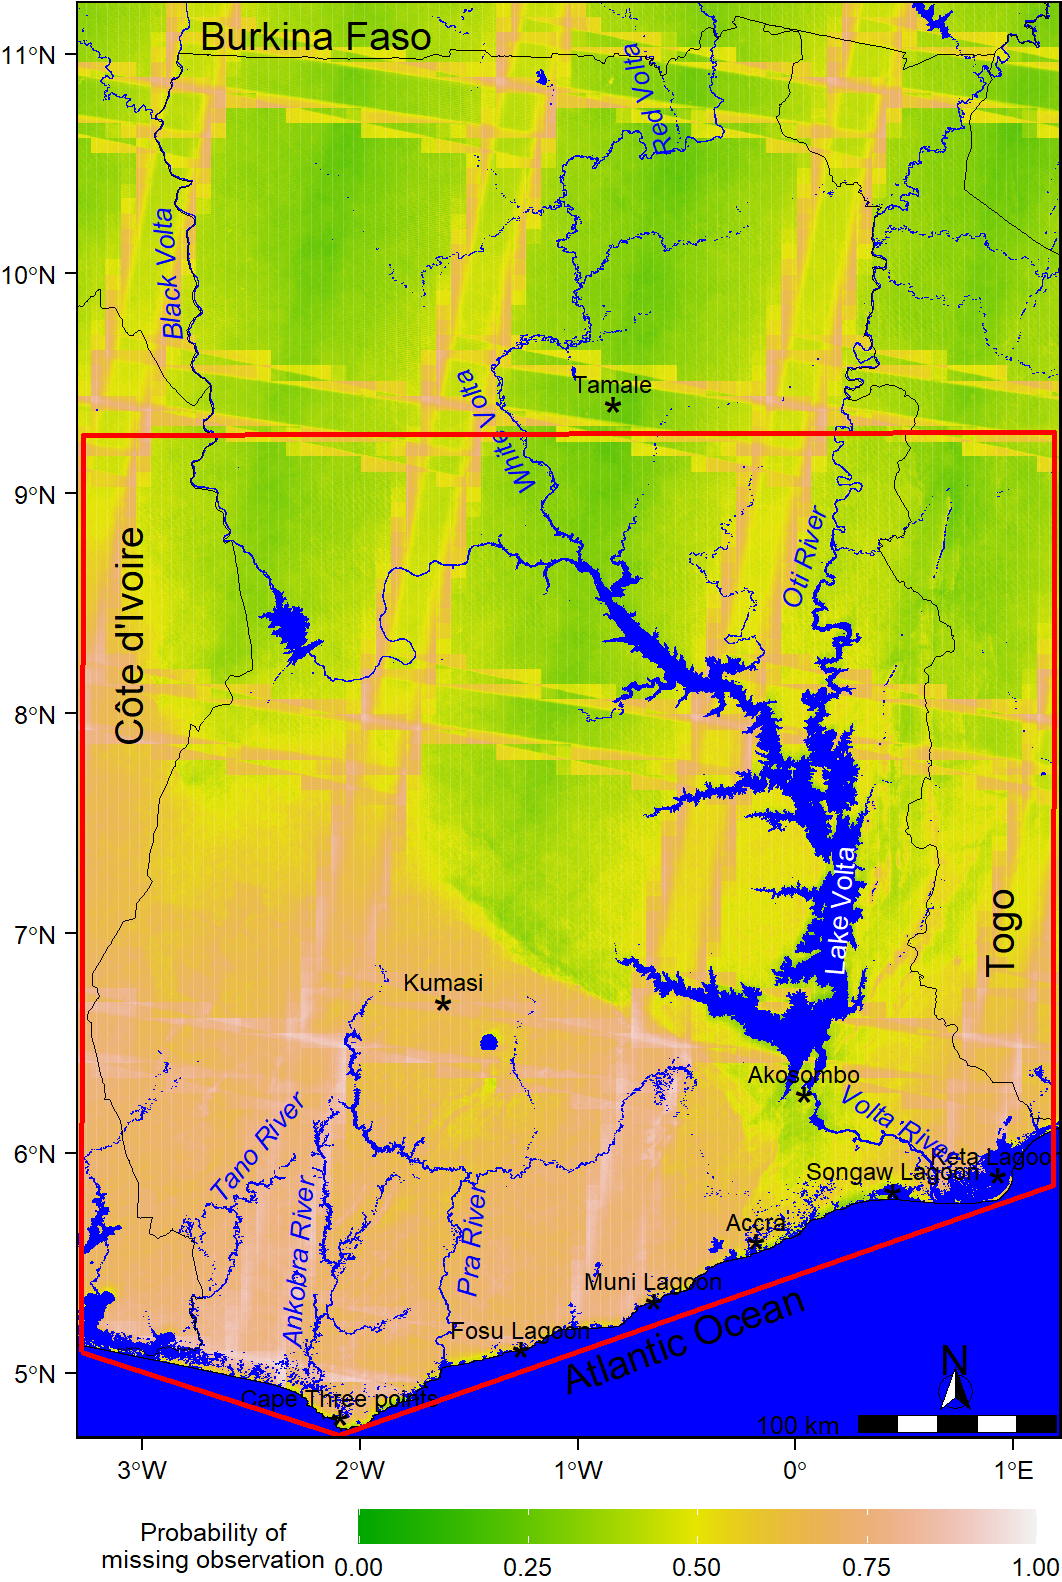
\includegraphics[width=0.5\linewidth,]{figures/pngs/Ghana_study_area_map} 

}

\caption{Major features and probability of missing data in Landsat collection between 1999 and 2020 in Ghana. The red box represents an area of interest and sampling frame for a spatial analysis of mangroves in Ghana. The probability of missing observation is estimated, as the ratio between the total number of missing data and the total number of acquisitions, based on all remote sensing artifacts as identified by Fmask algorithm.}\label{fig:fig1}
\end{figure}

\noindent rich body of fresh, and salty waters among which the major
ones include the red Volta, the Black Volta and the White Volta rivers
that originate in Burkina Faso to flow into Lake Volta and its estuary
(Figure \ref{fig:fig1}). Ghana has a coastline of about 550 km and over
100 estuaries and lagoons \citep{Levy-et-al-2015}.

As of 2010, the population of Ghana is estimated at nearly 25 million,
with an annual population growth rate of 3.1 per annum
\citep{Ghana-Statistical-Services-2012}. The coastal regions (e.g.,
Accra, Cape Coast) have the highest population density
\citep{Addae-and-Oppelt-2019}. These coastal regions experience two
rainy seasons between March to July and September to November, with an
annual average temperature of about 26.8 \(^\circ\)C. The monthly
temperature ranges from 24.7 \(^\circ\)C in August to 33 \(^\circ\)C in
March. While Landsat remained the publicly available source of data that
provides the best compromise between spatial and temporal resolutions in
Ghana until Sentinel data become available in 2015, the persistence of
cloud poses an important problem for optical remote sensing application
\citep{Ashiagbor-et-al-2021}. The chance of obtaining a clear
observation at a given pixel rarely exceed 0.5, particularly in the
coastal region (Figure \ref{fig:fig1}). This limits the amount of usable
data \citep{Ashiagbor-et-al-2021}, making it difficult to map the entire
landscape. This is a region of intensive LULC changes due to
anthropogenic activities. Most of these changes, however, are gradual,
meaning that the phenology of LULC remains more or less stable over a
relatively short period (e.g., 2 to 3 years). For pixels where remote
sensing data are available, this phenology can be easily described using
time series statistical models.

In these areas, mangroves play important roles (e.g.~habitat for various
migratory birds and fish species, fishing ground, timber for
construction, wood fuel, herbal medicine, spiritual places) for rural
livelihood
\citep{Armah-et-al-2005, Spalding-et-al-1997, Spalding-et-al-2010, UNEP-2007}.
A decade ago, the total area of mangroves in Ghana ranged between 137
km2 and 140 km2 \citep{Armah-et-al-2009, UNEP-2007}. In Ghana, mangroves
are generally found around lagoons all over the coastline and Volta
River Estuary (Figure \ref{fig:fig1}). The most developed are found on
the west coast (Côte d'Ivoire border to Cape Three Points)
\citep{Spalding-et-al-1997}. Their distribution appears to follow the
gradient of salinity, with \emph{Rhizophora} species encountered around
open lagoons whereas species such as \emph{Avicennia germinans},
\emph{Conocarpus erectus}, \emph{Laguncularia racemosa} and
\emph{Acrostichum aureum} are found around closed lagoons
\citep{Spalding-et-al-1997}. While mangroves play key roles in the
coastal regions of Ghana, existing studies of mangroves in Ghana appear
to generally concur with net declines in mangrove vegetation cover
across the country.

Ghana has a reach body of LULC (e.g., water bodies, forests, savannas,
shrublands, croplands), which are difficult to discriminate due to the
important cloud cover, particularly in the coastal regions (Figure
\ref{fig:fig1}). To accurately capture all mangroves vegetation and its
dynamics, we considered all major LULC considering the whole country
from East to West on a section spanning from the Atlantic Ocean to
latitude 9.23 (Figure \ref{fig:fig1}; red box). Our area of interest
covers the Worldwide Reference System Path 192 to 196 and Row 053 to
057.

\hypertarget{satellite-imageries}{%
\subsection{Satellite imageries}\label{satellite-imageries}}

To consistently capture the phenology of LULC and provide accurate
estimates of mangroves in Ghana, we considered all Landsat Tiers 1 and
Tiers 2 collections, available

\begin{figure}[!htbp]

{\centering 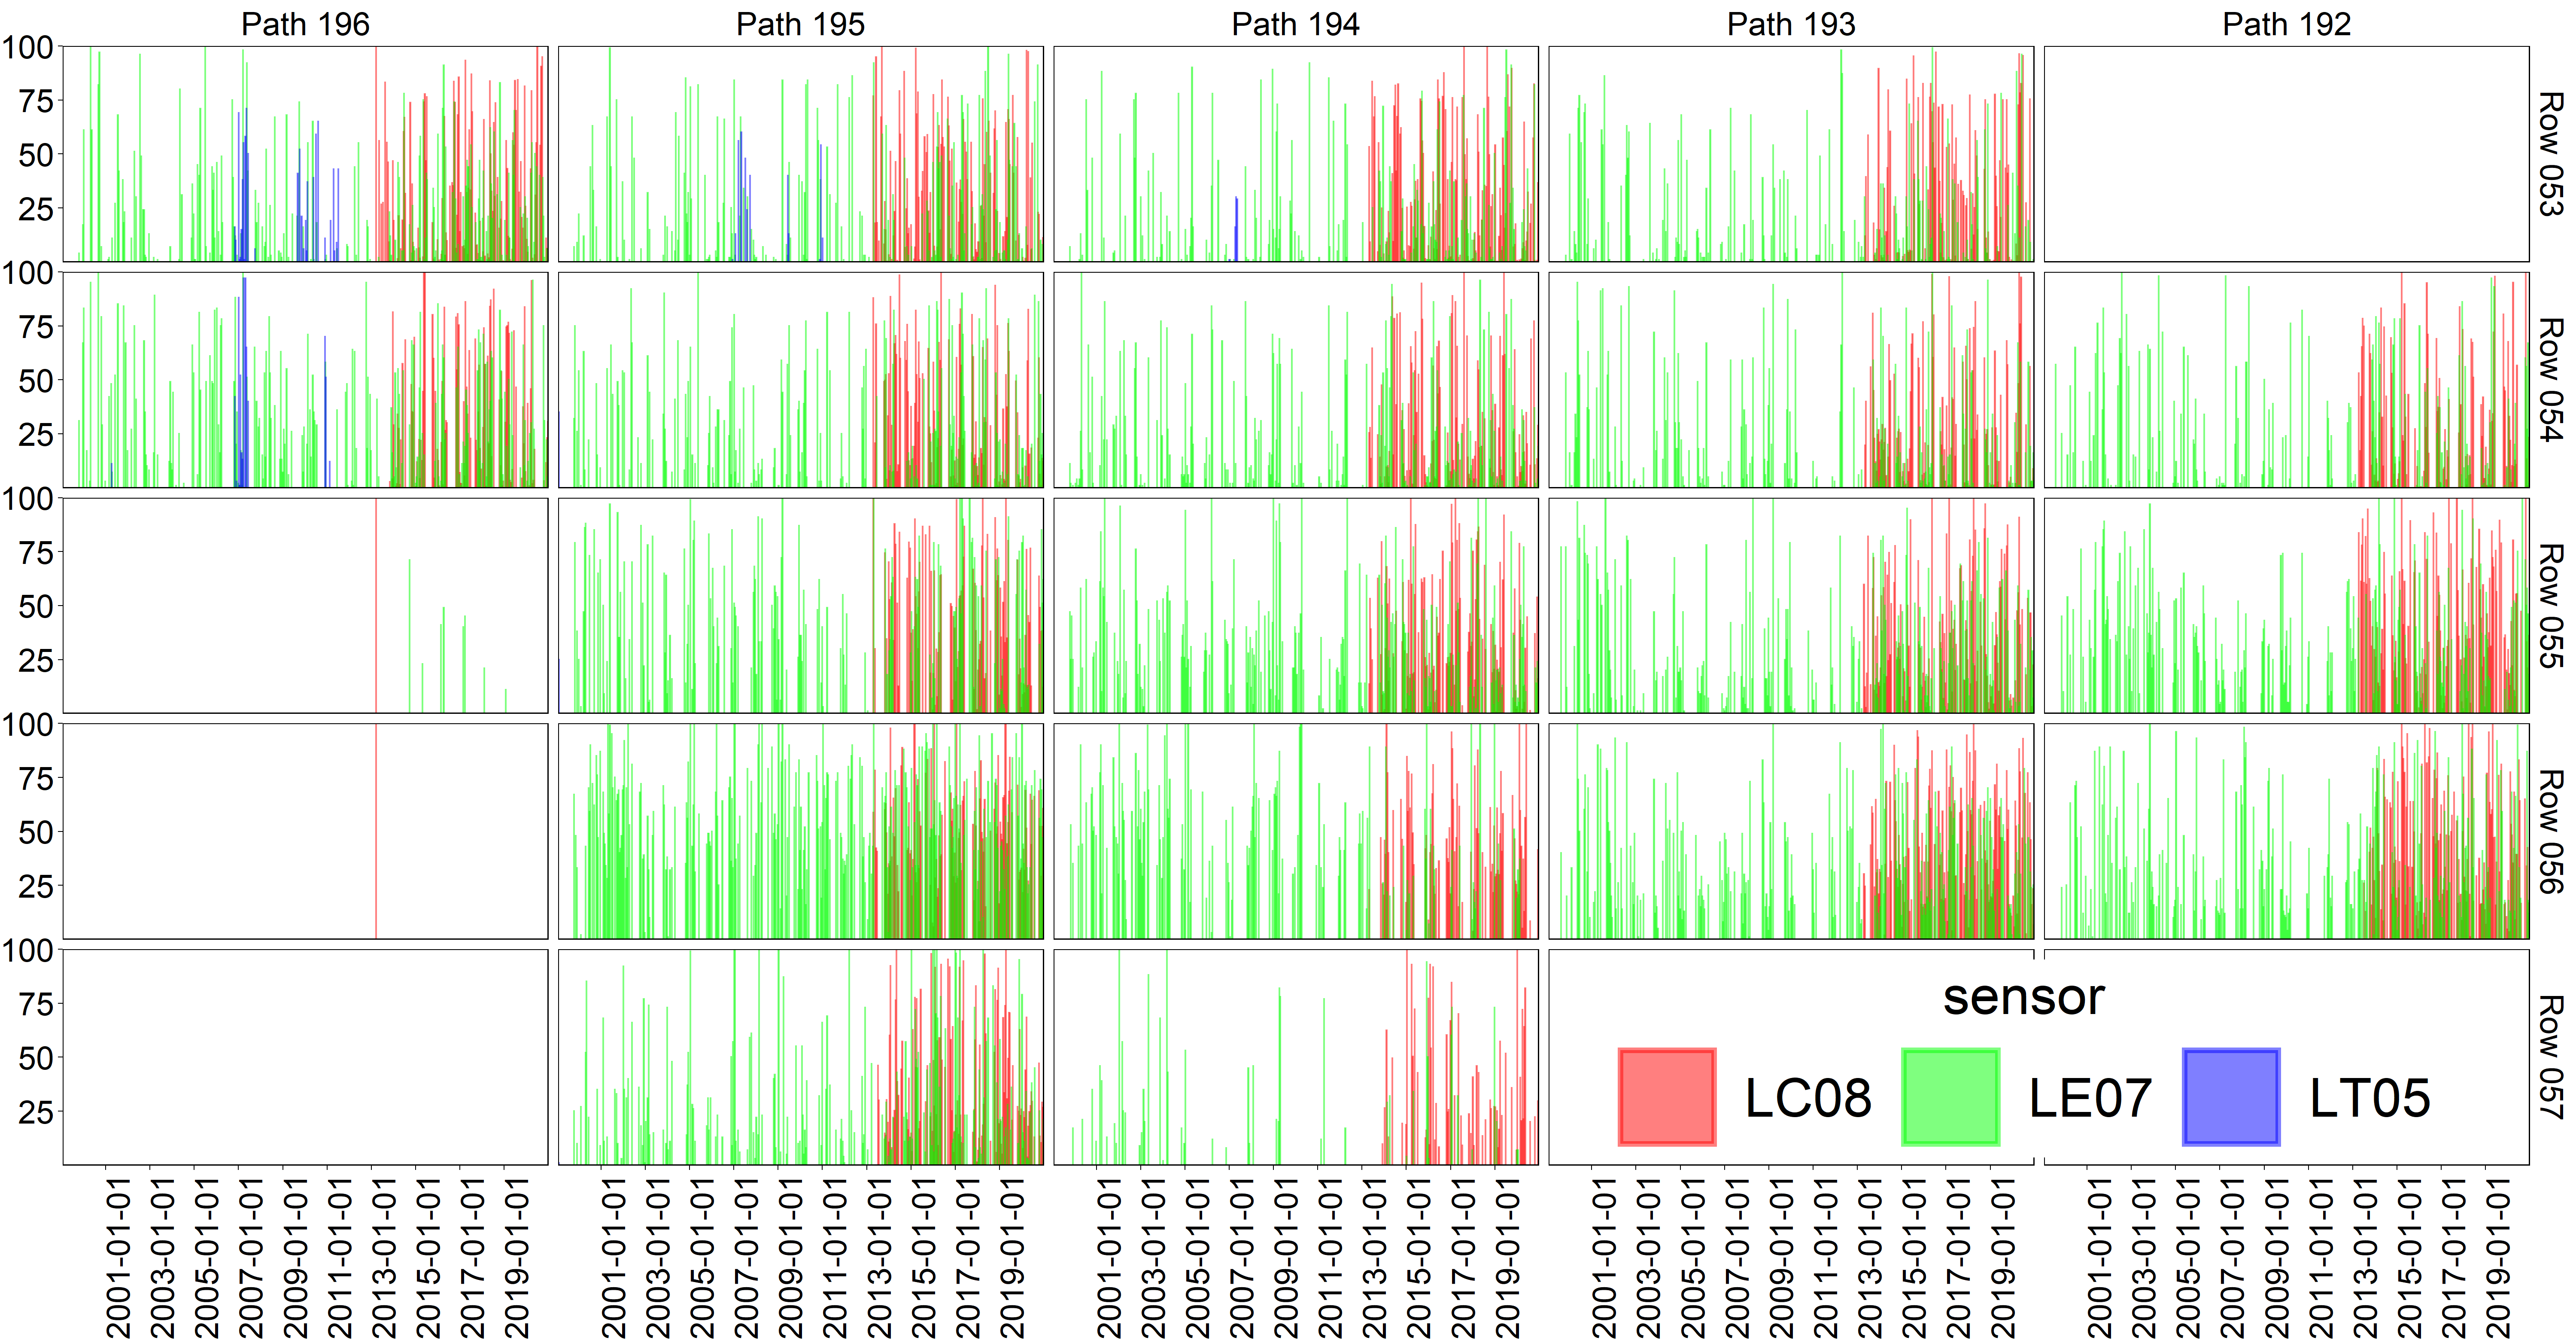
\includegraphics[width=1\linewidth,]{figures/pngs/Ghana_CloudScore} 

}

\caption{Percent cloud cover of Landsat collection in Ghana between 1999 and 2000. The acronyms in the legend represent the different Landsat sensors, with LC08 for Landsat 8 OLI - TIRS (Operational Land Imager and Thermal Infrared Sensor), LE07 for Landsat 7 Enhanced Thematic Mapper Plus and LT05 for Landsat 5 Thematic Mapper}\label{fig:fig2}
\end{figure}

\noindent from Google Earth Engine cloud computing platform
\citep{Gorelick-et-al-2017, Wulder-et-al-2019}, acquired between 1999
and 2020. We used a total number of 6409 Landsat tiles, each of which
composed of 6 bands covering the 3 visible bands, the near infrared
band, and the 2 short wave infrared bands. We considered the blue (0.45
- \SI{0.52}{\micro\metre}), the green (0.52 - \SI{0.60}{\micro\metre}),
the red (0.63 - \SI{0.69}{\micro\metre}), the near infrared or NIR (0.77
- \SI{0.90}{\micro\metre}), the shortest wave infrared or SWIR1 (1.55 -
\SI{1.75}{\micro\metre}) and the longest wave infrared or SWIR2 (2.09 -
\SI{2.35}{\micro\metre}) Landsat channels to account for different
frequency ranges along the electromagnetic spectrum in relation to
differences in the reflectance of LULC. These atmospherically corrected
data are suitable for LULC analysis since the surface reflectance values
are comparable to those measured on the ground. They are also good
candidates for change detection because they account for major
atmospheric factors such as clouds, cloud shadow and aerosol scattering.

Cloud and cloud shadow are the main factor limiting the amount of usable
Landsat images in the study area (Figure \ref{fig:fig1}; Figure
\ref{fig:fig2}). While cloud cover often reaches 100 \% in most areas of
Ghana, the coastal regions appear to be the cloudiest (Figure
\ref{fig:fig1}). Cloud cover appears to persist throughout the year over
the rows 055 and 056, with the path 195 being the most affected. We
noted that nor Tiers 1 neither Tiers 2 data from Landsat 4 Thematic
Mapper are available between 1999 and 2020 over Ghana. Only 85 images
were available from Landsat 5 Thematic Mapper over the area of interest.
This gap in Landsat data suggests that some gap filling may be required
when considering continuous time series of Landsat data in the region.

Prior to image classification, we removed all cloudy observations,
harmonized the data across sensors, mosaic the tiles based on monthly
(30 days) median composites, removed the noisy data, filled in the
missing ones, and recover the main signal for each pixel (see section
\ref{ref41}) for more details) for details). We assume that LULC remain
essentially unchanged over a relatively short period (e.g., 3 years) in
the area of interest and considered 3 reference periods for image
classification. These are the period 2000 -- 2002, the period 2010 --
2012, and the period 2018 -- 2020. We will refer to these as 2000, 2010
and 2020 and their respective classifications as 2000-classification,
2010-classification and 2020-classification.

\hypertarget{considerations-for-data-inputs-and-image-classification}{%
\subsection{Considerations for data inputs and image
classification}\label{considerations-for-data-inputs-and-image-classification}}

We conducted extensive field survey to identify 17 LULC classes based on
which we systematic ally collected reference data for training and
validation of LULC classifications. To provide a comprehensive LULC
nomenclature, we defined most of these LULC classes (Table \ref{tab1})
based on the standard IGBP and FAO LULC classification systems
\citep{Di-Gregorio-et-al-2016, FRA-2000}.

\begin{table}[H]

\caption{\label{tab:tab1}\label{tab1}Categories of land use and land cover used for an image classification in Ghana.}
\centering
\resizebox{\linewidth}{!}{
\begin{threeparttable}
\begin{tabular}[t]{l>{\raggedright\arraybackslash}p{35em}r}
\toprule
\textbf{Standard class} & \textbf{Class description} & \textbf{Map legend}\\
\midrule
Water bodies & Natural and artificial Water bodies such as ocean, rivers, and other reservoirs containing fresh or salty water for the most period of the year. & Waters\\
\addlinespace
Closed forests & Lands dominated by trees with a percent cover greater than 70 \% during the entire period of the year. & Closed forests\\
\addlinespace
Open forests & Lands dominated by trees with a percent cover between 60 and 70 \% during the entire period of the year. & Open forests\\
\addlinespace
Woody savannas & Lands with herbaceous and other understory systems, and with forest canopy cover between 30\% and 60\%.The forest cover height exceeds 2 m. & Woody savannas\\
\addlinespace
Savannas & Lands with herbaceous and other understory systems, and with forest canopy cover between 10\% and 30\%. The forest cover height exceeds 2 m. & Savannas\\
\addlinespace
Closed shrublands & Lands with woody vegetation less than 2 m tall and with shrub canopy cover > 60\%. The shrub foliage can be either evergreen or deciduous. & Closed shrublands\\
\addlinespace
Open shrublands & Lands with woody vegetation less than 2 m tall and with shrub canopy cover between 10\% and 60\%. The shrub foliage can be either evergreen or deciduous. & Open shrublands\\
\addlinespace
Grasslands & Lands with herbaceous types of cover. Tree and shrub cover is less than 10\%. & Grasslands\\
\addlinespace
Permanent wetlands & Lands with a permanent mixture of fresh water and herbaceous or woody vegetation. & Wetlands\\
\addlinespace
Croplands & Lands covered with temporary crops followed by harvest and a bare soil period (e.g., single and multiple cropping systems). & Croplands\\
\addlinespace
Urban and built-up lands & Land covered by buildings and other man-made structures. This class includes all concrete cover, such as roads. & Built-up\\
\addlinespace
Cropland and natural vegetation mosaics & Lands with a mosaic of croplands, forests, shrubland, and grasslands in which no one component comprises more than 60\% of the landscape. & Mosaics\\
\addlinespace
Barren & Lands with exposed soil, sand, rocks, or snow and never have more than 10\% vegetated cover during any time of the year. & Barren\\
\addlinespace
Mangroves & Lands with a permanent mixture of brackish water and herbaceous or woody vegetation. & Mangroves\\
\addlinespace
Salt mines & Land with water of high salt concentration where the salt naturally emerges or is artificially extracted from evaporite formations. & Salt mines\\
\addlinespace
Tree plantations & Land with perennial crop in the form of artificial forests. These are mostly represented by palm trees in the coastal region of Ghana. & Tree plantations\\
\addlinespace
Regularly Flooded vegetation & Land transitioning between terrestrial and fresh water zones with sufficient moisture for the development of near evergreen vegetation. & Riparian vegetation\\
\bottomrule
\end{tabular}
\begin{tablenotes}
\item \textit{Note: } 
\item Regularly Flooded Vegetation, closed forests and open forests are based on FAO LULC classification system. Tree plantations are mostly represented by palm trees. The remaining classes are based on IGBP land cover classification system except for Mangroves which is the class of interest and Salt mines which is relevant in regards to mangroves vegetation dynamics in Ghana. Perennial woody crops are classified as either tree plantations (mostly palm trees) or the appropriate forest or shrub land cover type.
\end{tablenotes}
\end{threeparttable}}
\end{table}

The first step in the collection of the reference data consisted of
identifying regions of dominant LULC and collecting large polygons over
these regions. These reference polygons are distributed over the area of
interest in a way that captures the essential LULC variability (both
between and within class variability). The second step consisted of
identifying pixels of persistent LULC within each reference polygon and
extracting the reflectance values of these pixels from the multiband
image. Pixels of persistent LULC are pixels whose class remains
unchanged across the reference periods considered. We used these
persistent pixels to ensure that the reflectance values used for
training and validation are consistent with the phenology of their
corresponding LULC across the reference periods.

The identification of the reference points involved the use of
unsupervised classifications. For each reference period, we randomly
sampled 1000 points and used k means clustering algorithm to classify
the image time series into 17 classes. We then identified the LULC
classes based on the reference polygons which also served as spatial
bounding boxes for sampling the reference points. We used stratified
random sampling to extract the reflectance values of the image time
series over 700 reference points for each of the 17 classes. This
required careful visual observation and matching of class configurations
across the entire landscapes of the classified images.

\hypertarget{methods}{%
\section{Methods}\label{methods}}

\hypertarget{ref41}{%
\subsection{Image pre-processing}\label{ref41}}

Prior to image classifications, we conducted a number of tasks to
minimize the effects of external factors on the resulting LULC
classification. These image pre-processing tasks involved several steps
including the masking of cloudy pixels, the scaling of reflectance
values across the different Landsat sensors, the removal of noisy data,
gap filling, and the processing of the phenological signal. We used the
quality assessment band provided along with the surface reflectance
product to mask all cloudy pixels. Despite the similarity of Landsat
sensors, data from different sensors present a slight difference which
can be relevant for analysis involving multiple sensors such as
cross-sensor time series, temporal image composite, or gap filling.
Therefore, we scaled the reflectance to the value range of OLI sensor
using the harmonisation coefficients provided by \citet{Roy-et-al-2016}.

\begin{mdframed}
\begin{flalign}
&\begin{aligned}
p_t &= \beta_0 + \beta_1 t + Acos(2\pi\omega t +\varphi) + e_t \footnotesize\text{ (Non-linear form)}\\
&= \beta_0 + \beta_1 t + \beta_2 cos(2\pi\omega t) + \beta_3 sin(2\pi\omega t) + e_t \footnotesize\text{ (Linearized form)}\\
&\text{Where,}\\
&\footnotesize\circ\text{$\beta_0$ is the intercept (Starting point of $p$)}\\
&\footnotesize\circ\text{$\beta_1$ is the slope (How fast $p$ changes with time)}\\
&\footnotesize\circ\text{$t$ is the time indexed at $t_0,t_1,\dots,t_N$ (Time since the epoch in radians)}\\
&\footnotesize\circ\text{$A$ is the amplitude (The peak)}\\
&\footnotesize\circ\text{$\omega$ is the frequency of oscillation ($\omega = 1$ for a single cycle)}\\
&\footnotesize\circ\text{$\varphi$ is a phase shift (Time at which $p$ reaches its peak)}\\
&\footnotesize\circ\text{$\beta_1 t$ is then,the linear term (Inter-annual variability)}\\
&\footnotesize\circ\text{$Acos(2\pi\omega t +\varphi)$  is  then, the harmonic term (Main signal as sinusoidal waveform)}\\
&\footnotesize\circ\text{$e_t$ is the random noise}\\
&\footnotesize\circ\text{$p_t$ is the predicted pixel value at time $t$}\\
&\footnotesize\circ\text{$\beta_2$, $\beta_3$ are the harmonic coefficients (Intra-annual variability)}\\
&\text{With,}\\
&\footnotesize\circ\text{$\beta_2 = Acos(\varphi)$}\\
&\footnotesize\circ\text{$\beta_3 = - Asin(\varphi)$}\\
&\footnotesize\circ\text{$A = (\beta_2^2 + \beta_3^2)^{1/2}$}\\
&\footnotesize\circ\text{$\varphi = \tan^{-1}(\beta_3 / \beta_2)$}\\
&\footnotesize\circ\text{$Acos(2\pi\omega t +\varphi) = \beta_2 cos(2\pi\omega t) + \beta_3 sin(2\pi\omega t)$} \label{eq:1}
\end{aligned}&&
\end{flalign}
\end{mdframed}

Despite the recent improvements and its widespread use, the Fmask
algorithm used to derive the quality assessment band in Landsat surface
reflectance product has its limitations in that the algorithm may not
always detect cloudy pixels
\citep{Zhu-et-al-2015, Zhu-and-Woodcock-2014}. Therefore, we used
equation \eqref{eq:1} in a Robust Iteratively Reweighted Least Squares
(RIRLS) framework to identify and removed such noisy data along with
other outliers induced by erratic events (e.g., fire or flooding)
following the procedure described in \citet{Zhu-and-Woodcock-2014}. We
used sine and cosine functions to specify non-linear models whose
parameters depend on the temporal distribution of clear pixel values as
determined by Fmask algorithm (equation \eqref{eq:1}). Our approach
consisted in estimating the required parameters for models having a
seasonality component to estimate land surface reflectance across the 6
Landsat bands. This was done only for pixels having a minimum number of
15 clear observations. We consider 2 rainy seasons (i.e., \(\omega\) = 2
in equation \eqref{eq:1}) to account for the inherent phenology of
ecological systems in the study area (e.g., bimodal distribution of
rainfall and vegetation).

\begin{mdframed}
\begin{flalign}
&\begin{aligned}
&p_{(green, t)} - \overline{p}_{(green, t)_{RIRLS}} > 0.04\ \text{    OR    } p_{(SWIR1, t)} - \overline{p}_{(SWIR1, t)_{RIRLS}} < -0.04\\
&\text{Where,}\\
&\footnotesize\circ\text{$t$ is the time indexed at $t_0,t_1, \dots,t_N$ (Time since the epoch in radians)}\\
&\footnotesize\circ\text{$p_{(green, t)}$ is the observed pixel value of the green band at time t}\\
&\footnotesize\circ\text{$\overline{p}_{(green, t)_{RIRLS}}$ is the robust predicted pixel value of the green band at time t}\\
&\footnotesize\circ\text{$p_{(SWIR1, t)}$ is the observed pixel value of the SWIR1 band at time t}\\
&\footnotesize\circ\text{$\overline{p}_{(SWIR1, t)_{RIRLS}}$ is the robust predicted pixel value of the SWIR1 band at time t}\\
&\text{With,}\\
&\footnotesize\circ\text{The green band corresponding to band 3 (0.53 - \SI{0.59}{\micro\metre}) of Landsat 8 OLI-TIRS or band 2}\\
&\footnotesize\text{(0.52 - \SI{0.60}{\micro\metre}) of Landsat 7 ETM+ and Landsat 5 TM.}\\
&\footnotesize\circ\text{The SWIR1 band corresponding to band 6 (1.57 - \SI{1.65}{\micro\metre}) of Landsat 8 OLI-TIRS or band 5}\\ &\footnotesize\text{(1.55 - \SI{1.75}{\micro\metre}) of Landsat 7 ETM+ and Landsat 5 TM.}\\
&\footnotesize\circ\text{The robust predicted corresponding to the predicted pixel value using RIRLS} \label{eq:2}
\end{aligned}&&
\end{flalign}
\end{mdframed}

We first used the model to screen out and mask all noisy observations by
comparing the robust model estimates against the observed pixel values
\citep{Zhu-and-Woodcock-2014}. A pixel value is considered as noisy and
masked at any time step, when either the difference between the observed
and predicted pixel value of the green band is greater than 0.04 or the
difference between the observed and predicted pixel value of the
shortest wave infrared band is less than 0.04 (equation \eqref{eq:2}).

\begin{mdframed}
\begin{flalign}
&\begin{aligned}
p_{(x, t)_{missing}} &=
\begin{cases}
\overline{p}_{(x, t)_{RIRLS}}, if\\
\begin{cases}
p_{(green, t)} - \overline{p}_{(green, t)_{RIRLS}} \le 0.04\\
OR\\
p_{(SWIR1, t)} - \overline{p}_{(SWIR1, t)_{RIRLS}} \ge -0.04\\
\end{cases}\\
missing, otherwise\\
\end{cases}\\
&\text{Where,}\\
&\footnotesize\circ\text{$t$ is the time indexed at $t_0,t_1, \dots,t_N$ (Time since the epoch in radians)}\\
&\footnotesize\circ\text{$p_{(x, t)_{missing}}$ is the missing pixel value of the band $x$ at time $t$}\\
&\footnotesize\circ\text{$p_{(green, t)}$ is the observed pixel value of the green band at time $t$}\\
&\footnotesize\circ\text{$\overline{p}_{(green, t)_{RIRLS}}$ is the robust predicted pixel value of the green band at time $t$}\\
&\footnotesize\circ\text{$p_{(SWIR1, t)}$ is the observed pixel value of the SWIR1 band at time $t$}\\
&\footnotesize\circ\text{$\overline{p}_{(SWIR1, t)_{RIRLS}}$ is the robust predicted pixel value of the SWIR1 band at time $t$}\\
&\text{With,}\\
&\footnotesize\circ\text{The green band corresponding to band 3 (0.53 - \SI{0.59}{\micro\metre}) of Landsat 8 OLI-TIRS}\\
&\footnotesize\text{or band 2 (0.52 - \SI{0.60}{\micro\metre}) of Landsat 7 ETM+ and Landsat 5 TM.}\\
&\footnotesize\circ\text{The SWIR1 band corresponding to band 6 (1.57 - \SI{1.65}{\micro\metre}) of Landsat 8 OLI-TIRS}\\
&\footnotesize\text{or band 5 (1.55 - \SI{1.75}{\micro\metre}) of Landsat 7 ETM+ and Landsat 5 TM.}\\
&\footnotesize\circ\text{The robust predicted corresponding to the predicted pixel value using RIRLS} \label{eq:3}
\end{aligned}&&
\end{flalign}
\end{mdframed}

After identifying and removing the noisy observations, we used the
robust model estimates to replace all cloudy observations (equation
\eqref{eq:3}). Note that the noisy observations are kept missing at this
stage. To recover the phenological signal and remove all noises, we used
equation \eqref{eq:1} to fit an Ordinary Least Squares (OLS) model to
the gap-filled data and extracted the resulting signal which we used as
inputs for LULC classification.

\hypertarget{land-cover-classification-and-accuracy-assessment}{%
\subsection{Land cover classification and accuracy
assessment}\label{land-cover-classification-and-accuracy-assessment}}

The pre-processing of the land surface reflectance data resulted in a
collection of 267 multiband images where each band is a complete dataset
of monthly signal describing pixel phenology. From this large image
collection, we extracted the time series corresponding to each reference
period to make up a new sub-collection of 36 images, each of which
composed of 6 bands. The sub-collections were then flattened into a
single multiband image of 216 bands for image classifications.

Accuracy assessment is an important component of LULC classification and
any subsequent analysis. The first component of the accuracy assessment
consisted in estimating the performance of the harmonic model using the
root mean square error to illustrate how well does the model fit the
input data across different bands and LULC type. It is easy to produce
statistically accurate maps that do not reflect the real-world situation
due to inadequate validation samples (e.g., sample size and spatial
distribution). To provide the best accuracy assessment possible of the
LULC classification, we fairly evenly distributed our validation data,
cover most of the area of interest using a large sample, compute
statistical accuracy metrics using the traditional confusion matrix, and
used informal assessments using Google Earth imageries
(\url{https://www.google.com/earth/}) of high spatial and temporal
resolution. Giving more priority to validation than training, the 11,900
reference points were split into 30\% for training and 70\% for
validation. To conduct the LULC classification, we used a random forest
model with a maximum number of 100 trees for each reference period
\citep{Breiman-2001, Oshiro-2012}. The three classifiers have the same
specification and produce a similar statistical accuracy. To ensure the
best class separability and produce accurate results, we used these
classifiers to classify and validate the image times series
corresponding to their respective reference period.

\hypertarget{change-detection-in-land-cover}{%
\subsection{Change detection in land
cover}\label{change-detection-in-land-cover}}

Although mangroves are the main focus, we estimated the acreage of LULC
conversion across all the LULC classes involved in the classifications.
We compared the 2000-classification with the 2010-classification, the
2010-classification with the 2020-classifcation, and the
2000-classification with the 2020-classifcation to identify class
changes and compute the total areas of LULC change between these
reference periods in the area of interest. We then examined the changes
specifically involving mangrove vegetation. We screened the LULC
classifications of the 3 reference periods to identify all areas
classified at least once as mangroves to generate a mangrove mask which
we used to mask all non-mangrove pixels in the 3 classifications. Based
on the resulting masked classifications, we estimated the dynamics of
mangroves as decrease, stability, and increase in mangrove areas. Areas
of decrease are areas where mangroves vegetation were replaced with
other LULC as opposed to areas of increase, whereas areas of stability
are areas where mangrove vegetation persists.

\hypertarget{results}{%
\section{Results}\label{results}}

\hypertarget{evaluation-of-model-performance}{%
\subsection{Evaluation of model
performance}\label{evaluation-of-model-performance}}

The harmonic model appears to have generally captured the phenology of
the LULC across all the 6 Landsat bands with the majority of pixels
predicted with RMSE in the range of 300 (Figure \ref{fig:fig3}).
Relatively high RMSE are rare. The model appears to have achieved the
best performance over the short-wave infrared channels with the shortest
wave infrared being the best predicted. The model performance over the
shortest wave infrared appears to be comparable to that over the near
infrared. The model appears to have achieved, more or less similarly,
the lowest performance over the visible bands where difference across
tiles becomes more perceptible. In general, the model performance is
relatively poor over the coastal regions and areas of dense vegetation.
While water bodies appear to be essentially associated with the lowest
RMSE, this RMSE appears to slightly increase over riparian vegetation.
In general, the performance of the model appears to increase with
wavelength and seasonality.

\begin{figure}[!htbp]

{\centering 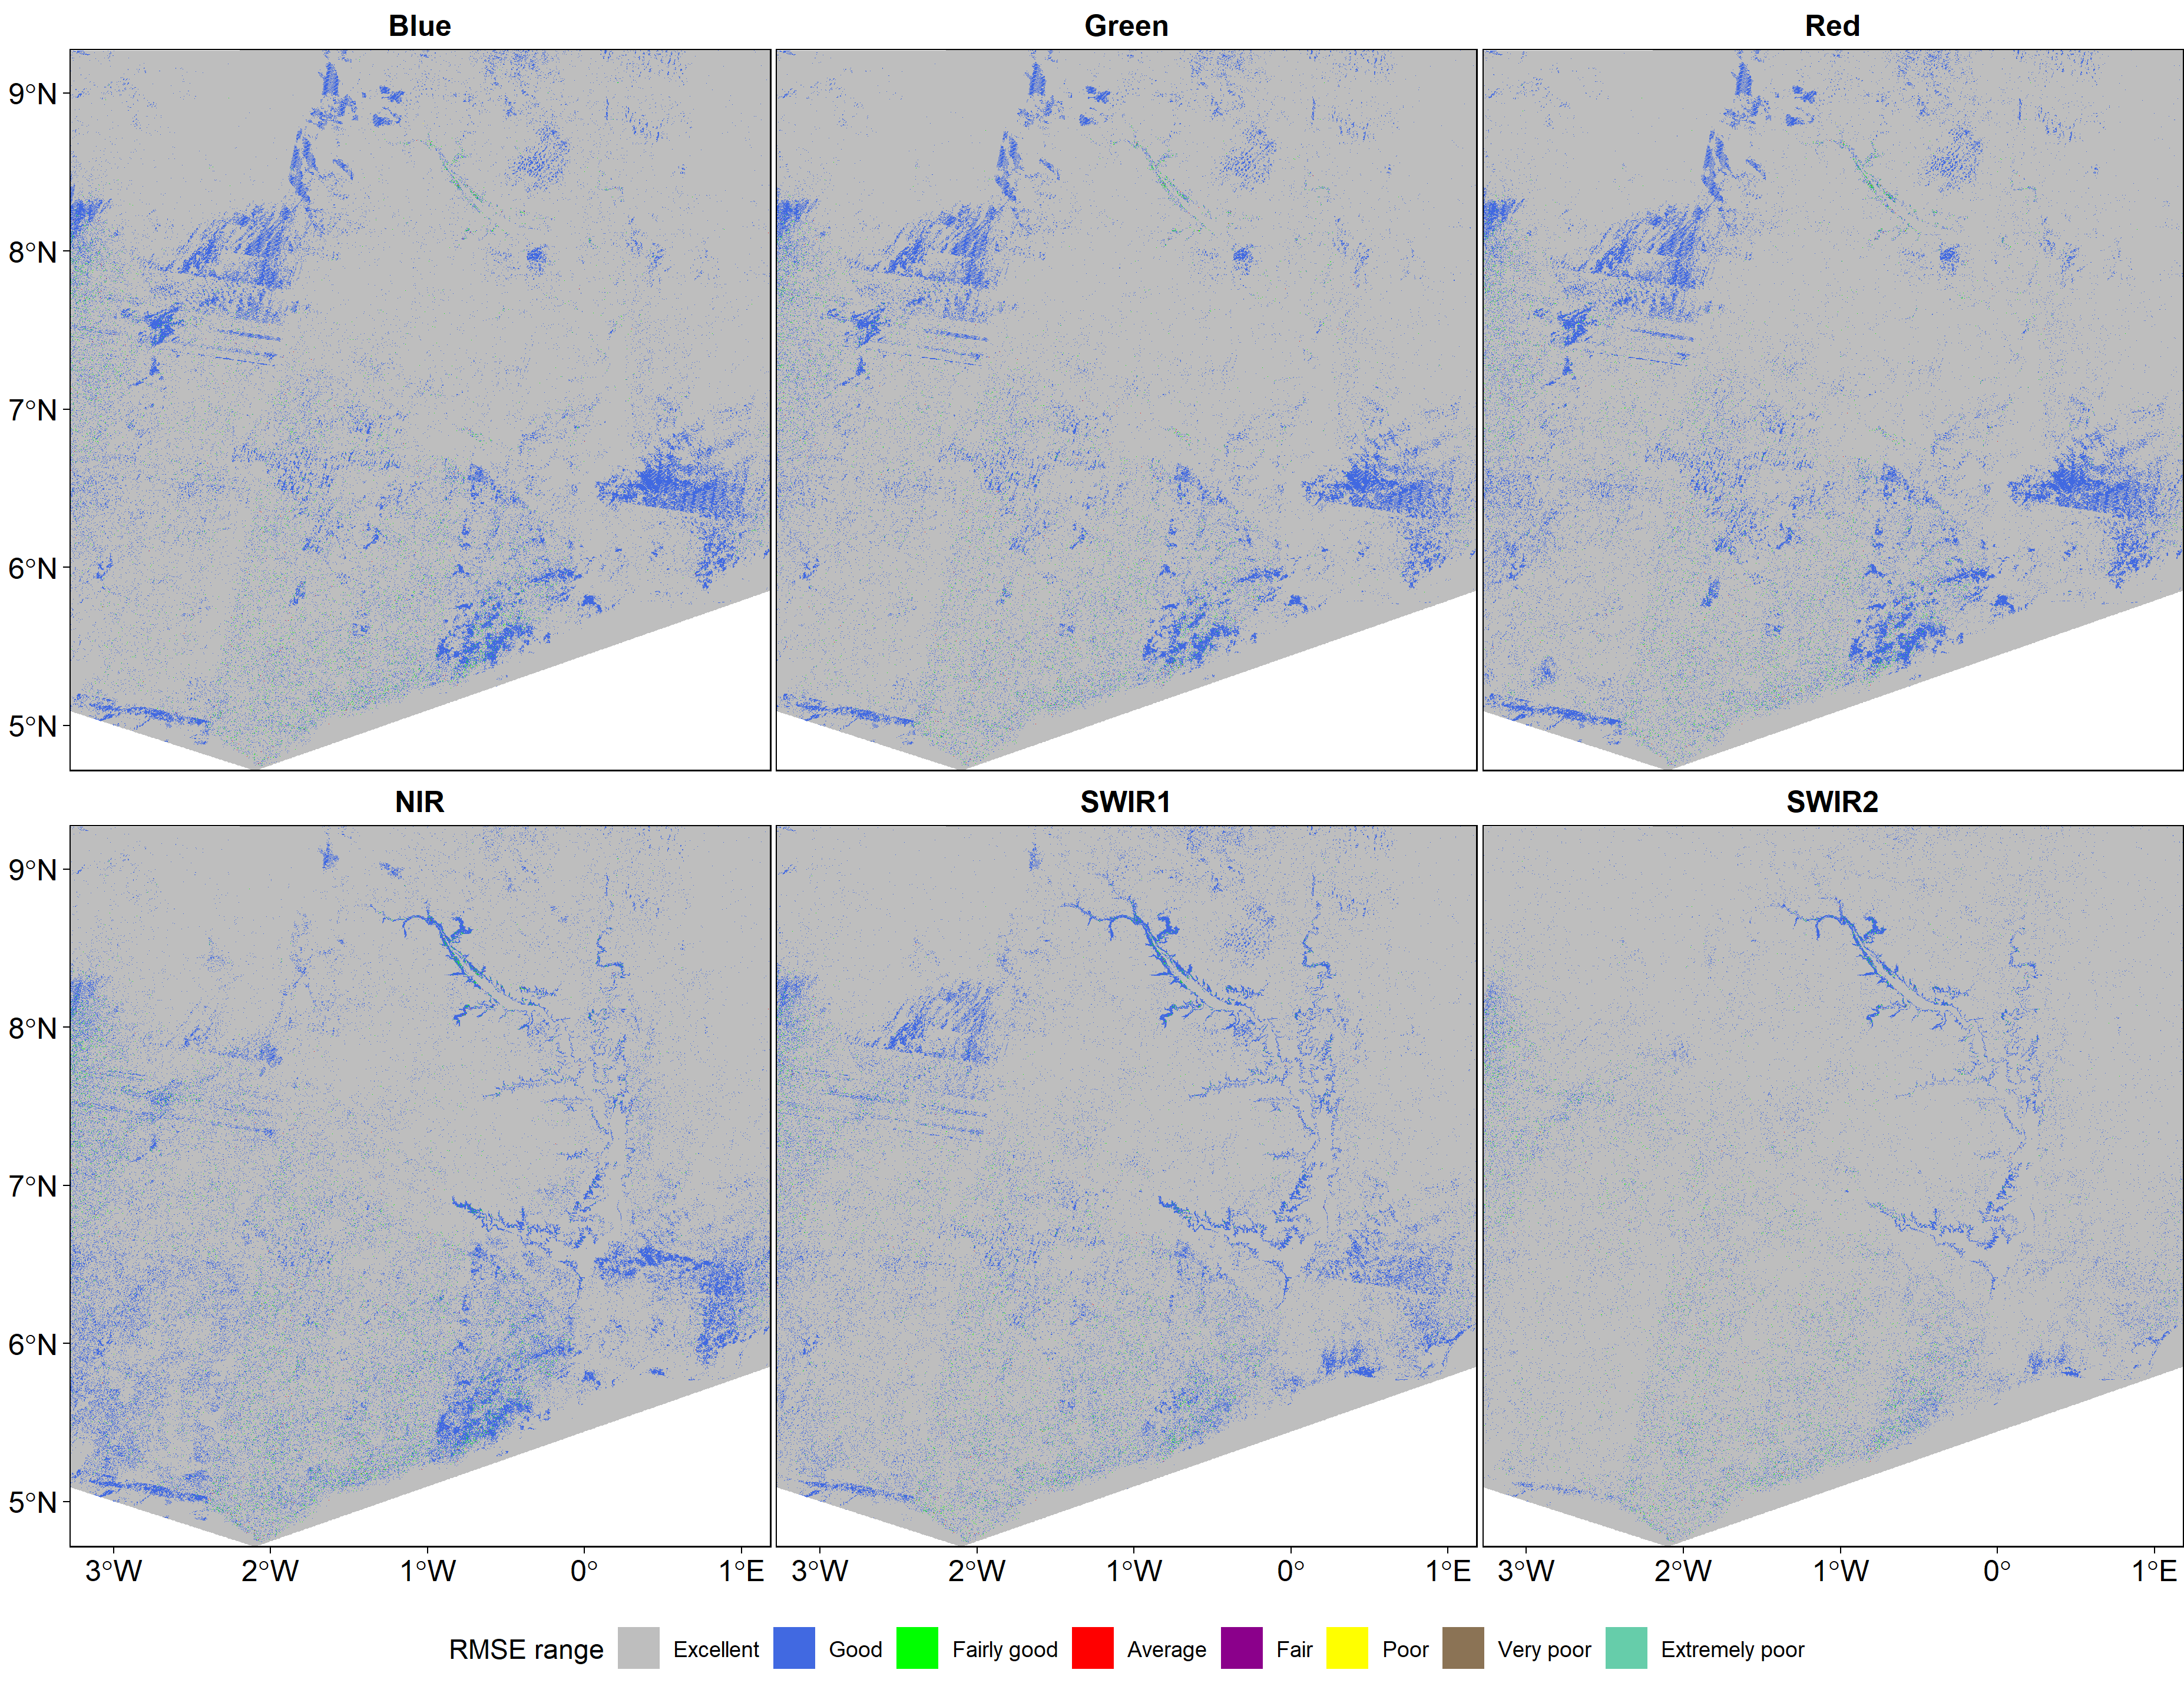
\includegraphics[width=1\linewidth,]{figures/pngs/Ghana_rmse_maps} 

}

\caption{Prediction error of a spatially explicit harmonic model fit to 6 bands of Landsat surface reflectance over Ghana. The prediction error is estimated as root mean square error (RMSE). The RMSE was grouped to improve visualisation based on \citet{Jiang-2013}'s head / tail breaks as implemented in classInt R package \citep{Bivand-2020}. The input data are in the range of thousands with the Likert scale in the legend corresponding to model performance and translating into the following RMSE range: Excellent = [0, 388[, Good = [388, 2990[, Fairly  good = [2990, 48600[, Average = [48600, 584000[, Fair = [584000, 5200000[, Poor = [5200000, 38200000[, Very poor = [38200000, 136000000[, Extremely poor = [136000000, 389000000[.}\label{fig:fig3}
\end{figure}

The model performed generally well across the 17 LULC (Figure
\ref{fig:fig4}). The model achieved the best performance over LULC of
medium vegetation density (i.e., savannas, shrublands and croplands).
Relatively densely vegetated LULC (i.e., forests, tree plantation and
riparian vegetation) and water bodies exhibit a slightly lower model
performance. The lowest model performance is associated with
non-vegetated LULC (i.e., barren, built-up) and marine LULC (i.e.,
mangroves and salt mines).

\begin{figure}[!htbp]

{\centering 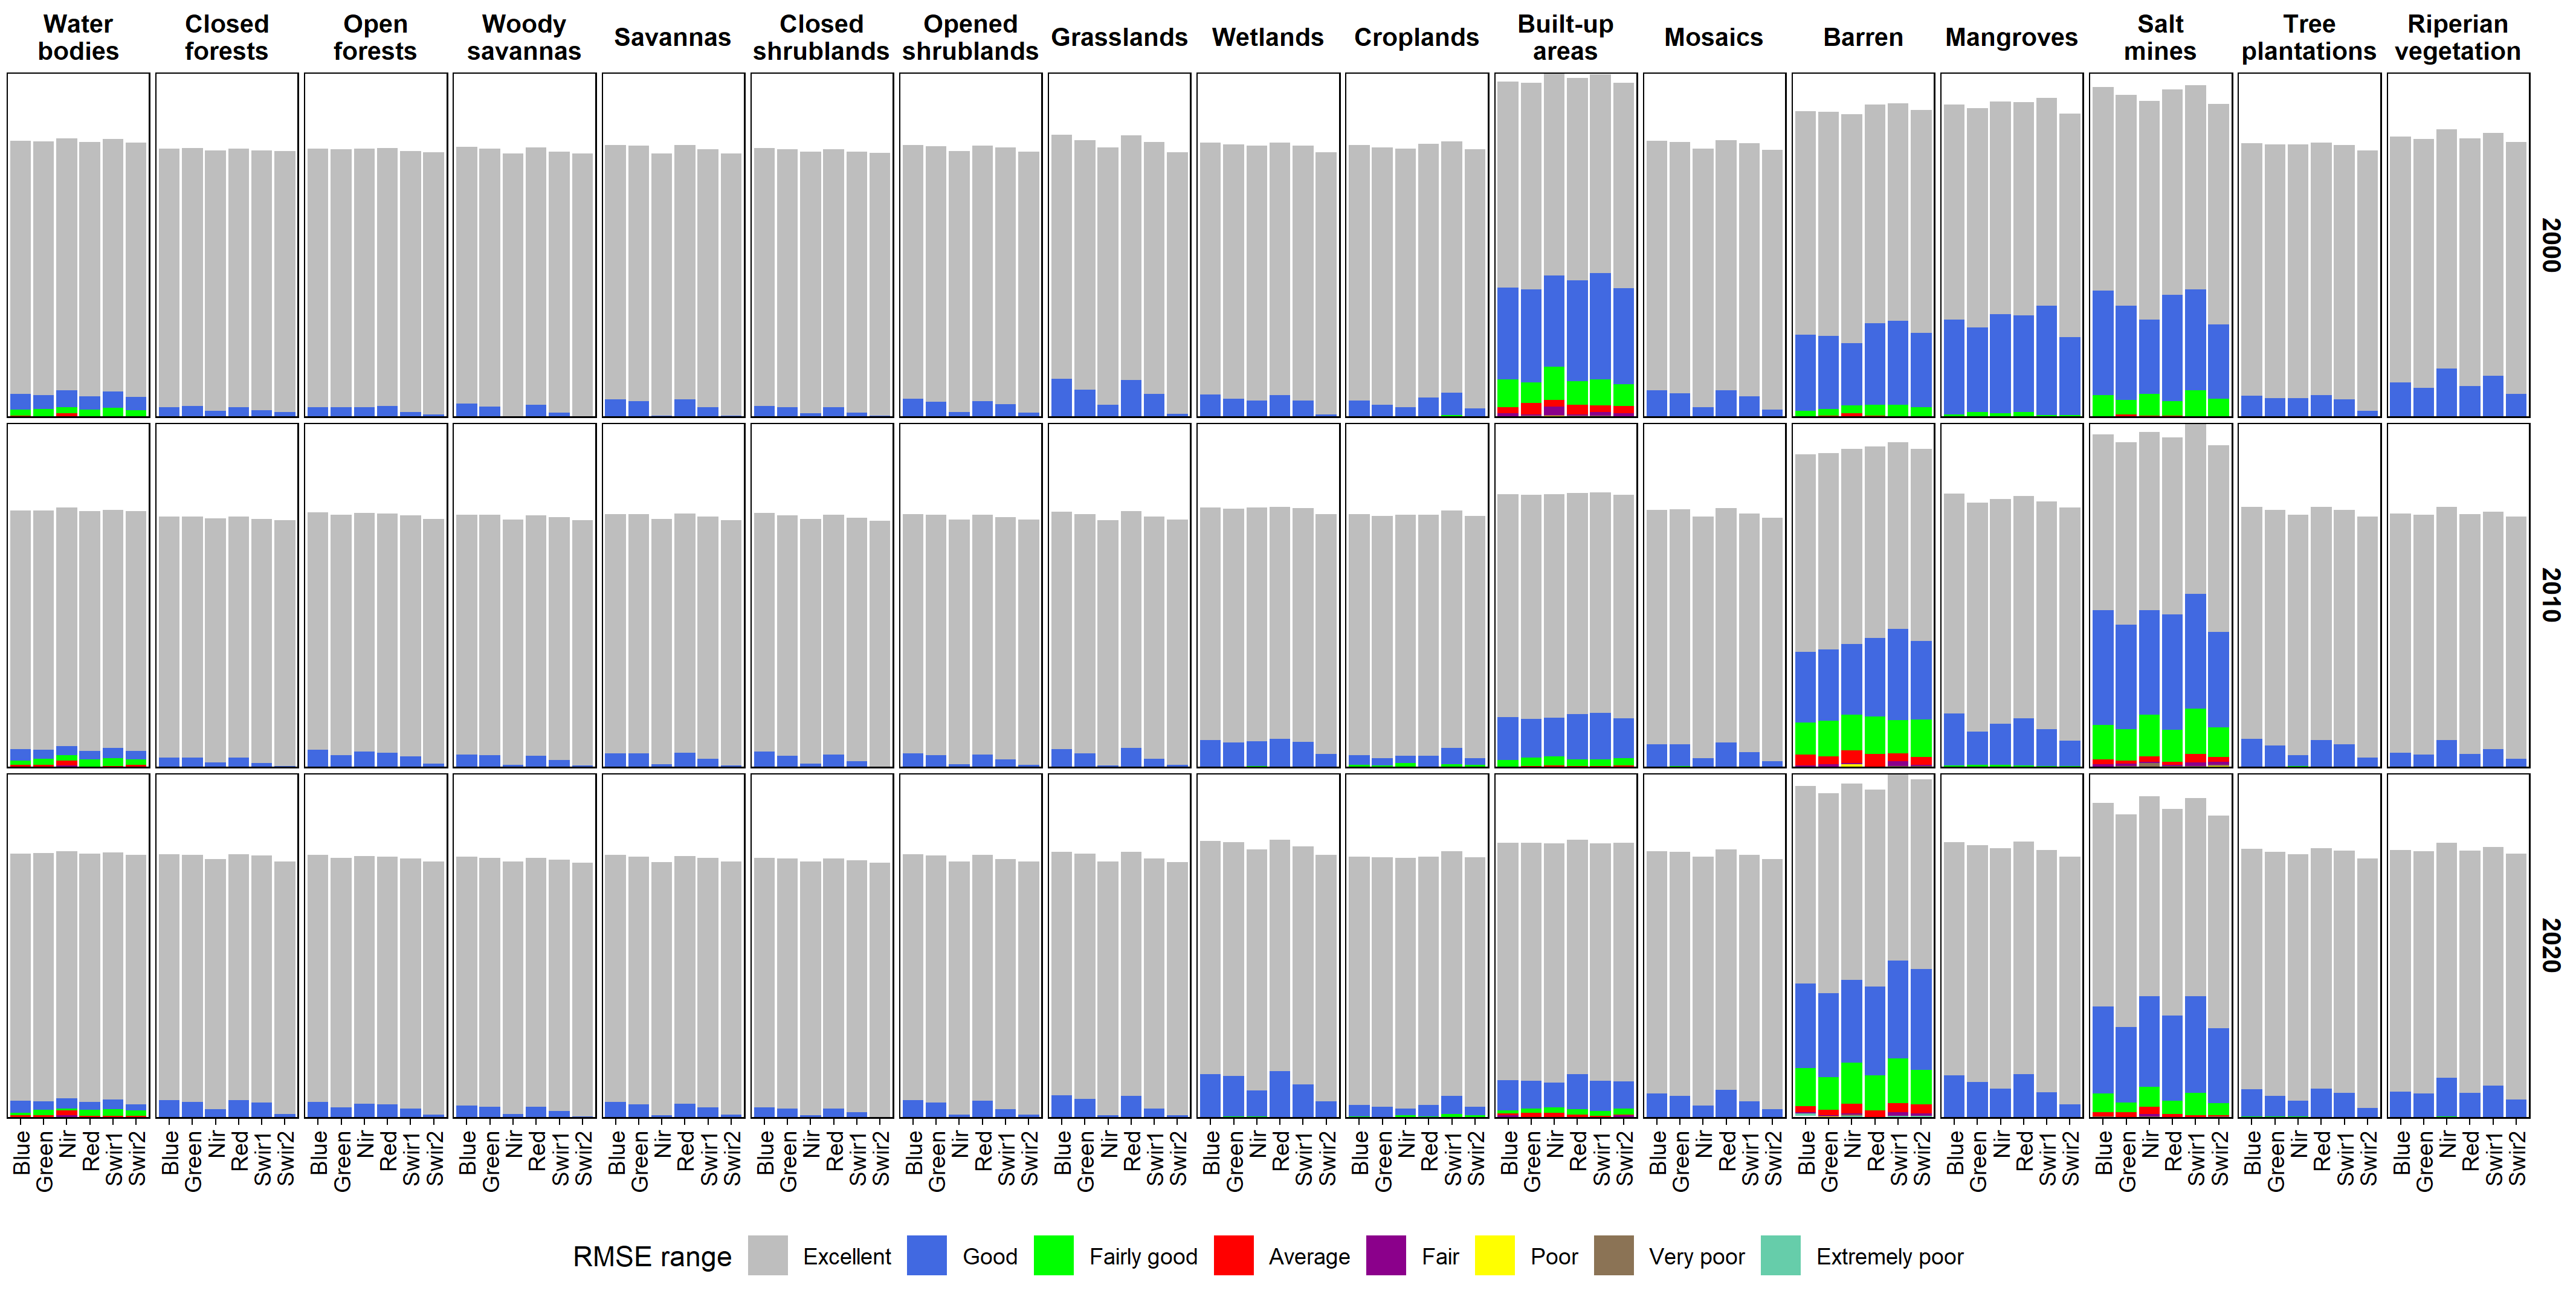
\includegraphics[width=1\linewidth,]{figures/pngs/Ghana_rmse_bars} 

}

\caption{Prediction error of a spatially explicit harmonic model across different land use and land cover in Ghana. The prediction error is estimated as root mean square error (RMSE). The RMSE was grouped to improve visualisation based on \citet{Jiang-2013}’s head / tail breaks as implemented in classInt R package \citep{Bivand-2020}. The input data are in the range of thousands with the Likert scale in the legend corresponding to model performance and translating into the following RMSE range: Excellent = [11.88, 681.24[, Good = [681.24, 7480.90[, Fairly  good = [7480.90, 66315.81[, Average = [48600, 354635.13[, Fair = [354635.13, 1253545.74[, Poor = [1253545.74, 2548527.97[, Very poor = [2548527.97, 4229437[.}\label{fig:fig4}
\end{figure}

The results of the statistical accuracy assessment conducted using the
confusion matrix approach show a minimum overall classification accuracy
of 94\% for 2020-classification and 2010-Classification, and a maximum
of 95\% for 2000-Classification. Kappa statistics range between 0.94 for
2020-classification to 0.95 for 2000-Classification (Table \ref{tab2}).
The accuracy for individual LULC classes ranges between 80\% and 100\%
for producer accuracy. These correspond to a minimum of 81\% and a
maximum of 100\% for consumer accuracy. The mangrove class was detected
with a producer accuracy ranging between 97\% and 98\%, and a consumer
accuracy ranging between 91\% and 97\%.

\begin{table}

\caption{\label{tab:tab2}\label{tab2}Statistical accuracy assessment of multitemporal land use and land cover classifications of southern Ghana conducted for mangrove vegetation analysis. The input data were pre-processed using time series statistical models via harmonic modelling of all available Tiers 1 and Tiers 2 Landsat surface reflectance data acquired between 2000 and 2020. This accuracy assessment is based on random forest classifiers with a maximum number of 100 trees.}
\centering
\resizebox{\linewidth}{!}{
\begin{tabular}[t]{>{\raggedright\arraybackslash}p{9em}>{\raggedleft\arraybackslash}p{5em}>{\raggedleft\arraybackslash}p{5em}>{\raggedleft\arraybackslash}p{5em}>{\raggedleft\arraybackslash}p{5em}>{\raggedleft\arraybackslash}p{5em}>{\raggedleft\arraybackslash}p{5em}>{\raggedleft\arraybackslash}p{5em}>{\raggedleft\arraybackslash}p{5em}>{\raggedleft\arraybackslash}p{5em}}
\toprule
\multicolumn{1}{c}{\textbf{ }} & \multicolumn{3}{c}{\textbf{2020-Classification}} & \multicolumn{3}{c}{\textbf{2010-Classification}} & \multicolumn{3}{c}{\textbf{2000-Classification}} \\
\cmidrule(l{3pt}r{3pt}){2-4} \cmidrule(l{3pt}r{3pt}){5-7} \cmidrule(l{3pt}r{3pt}){8-10}
\textbf{Land use and land cover class} & \textbf{Consumers accuracy} & \textbf{} & \textbf{Producer accuracy} & \textbf{Consumers accuracy} & \textbf{} & \textbf{Producer accuracy} & \textbf{Consumers accuracy} & \textbf{} & \textbf{Producer accuracy}\\
\midrule
Water bodies & 0.99 &  & 1.00 & 1.00 &  & 0.99 & 0.99 &  & 0.98\\
\addlinespace
Closed forests & 0.88 &  & 0.80 & 0.99 &  & 0.96 & 0.96 &  & 0.92\\
\addlinespace
Open forests & 0.98 &  & 0.99 & 0.91 &  & 0.91 & 0.97 &  & 0.96\\
\addlinespace
Woody savannas & 0.84 &  & 0.83 & 0.92 &  & 0.90 & 0.96 &  & 0.92\\
\addlinespace
Savannas & 0.96 &  & 0.97 & 0.82 &  & 0.85 & 0.96 &  & 0.99\\
\addlinespace
Closed shrublands & 0.99 &  & 0.96 & 0.85 &  & 0.82 & 0.94 &  & 0.92\\
\addlinespace
Opened shrublands & 0.99 &  & 0.99 & 1.00 &  & 0.99 & 0.98 &  & 0.99\\
\addlinespace
Grasslands & 0.98 &  & 0.98 & 1.00 &  & 0.99 & 0.98 &  & 0.96\\
\addlinespace
Wetlands & 0.81 &  & 0.84 & 0.89 &  & 0.91 & 0.88 &  & 0.93\\
\addlinespace
Croplands & 0.93 &  & 0.99 & 0.91 &  & 0.99 & 0.90 &  & 0.97\\
\addlinespace
Built-up areas & 0.93 &  & 0.90 & 0.94 &  & 0.88 & 0.92 &  & 0.85\\
\addlinespace
Mosaics & 0.98 &  & 0.99 & 0.98 &  & 1.00 & 0.95 &  & 0.93\\
\addlinespace
Barren & 0.94 &  & 0.91 & 0.95 &  & 0.93 & 0.95 &  & 0.95\\
\addlinespace
Mangroves & 0.96 &  & 0.97 & 0.97 &  & 0.98 & 0.91 &  & 0.98\\
\addlinespace
Salt mines & 0.99 &  & 0.99 & 0.99 &  & 1.00 & 0.99 &  & 1.00\\
\addlinespace
Tree plantations & 0.84 &  & 0.89 & 0.90 &  & 0.92 & 0.98 &  & 0.98\\
\addlinespace
Riperian vegetation & 0.97 &  & 0.99 & 0.99 &  & 1.00 & 0.99 &  & 0.96\\
\midrule
\addlinespace
Overall accuracy &  & 0.94 &  &  & 0.94 &  &  & 0.95 & \\
\addlinespace
Kappa &  & 0.94 &  &  & 0.94 &  &  & 0.95 & \\
\bottomrule
\end{tabular}}
\end{table}

Considering the number of classes (17 LULC classes), the even
distribution of the validation points, and the number of 500 validation
samples per class (8500 points in total), the results are satisfactory.
These are consistent with the informal accuracy assessment conducted
using the images from Google Earth. The classification appears to
accurately represent the configuration of LULC classes on the ground. In
some areas, however, it was not possible to track back these LULC
through time due to the lack of temporal Google Earth imagery.

\hypertarget{land-cover-changes}{%
\subsection{Land cover changes}\label{land-cover-changes}}

At glance, major features in the coastal regions of Ghana are the closed
forests encountered between 3\(^\circ\)W to 0\(^\circ\)W and
5\(^\circ\)N to 7\(^\circ\)N, the water bodies including the network of
Volta water bodies, the Atlantic Ocean, the built-up areas with major
cities such as Accra and Kumasi being more visible, the tree plantations
in the 2000-Classification, and the open forests in both the
2010-Classification and the 2020-Classification (Figure \ref{fig:fig5}).

\begin{figure}[!htbp]

{\centering 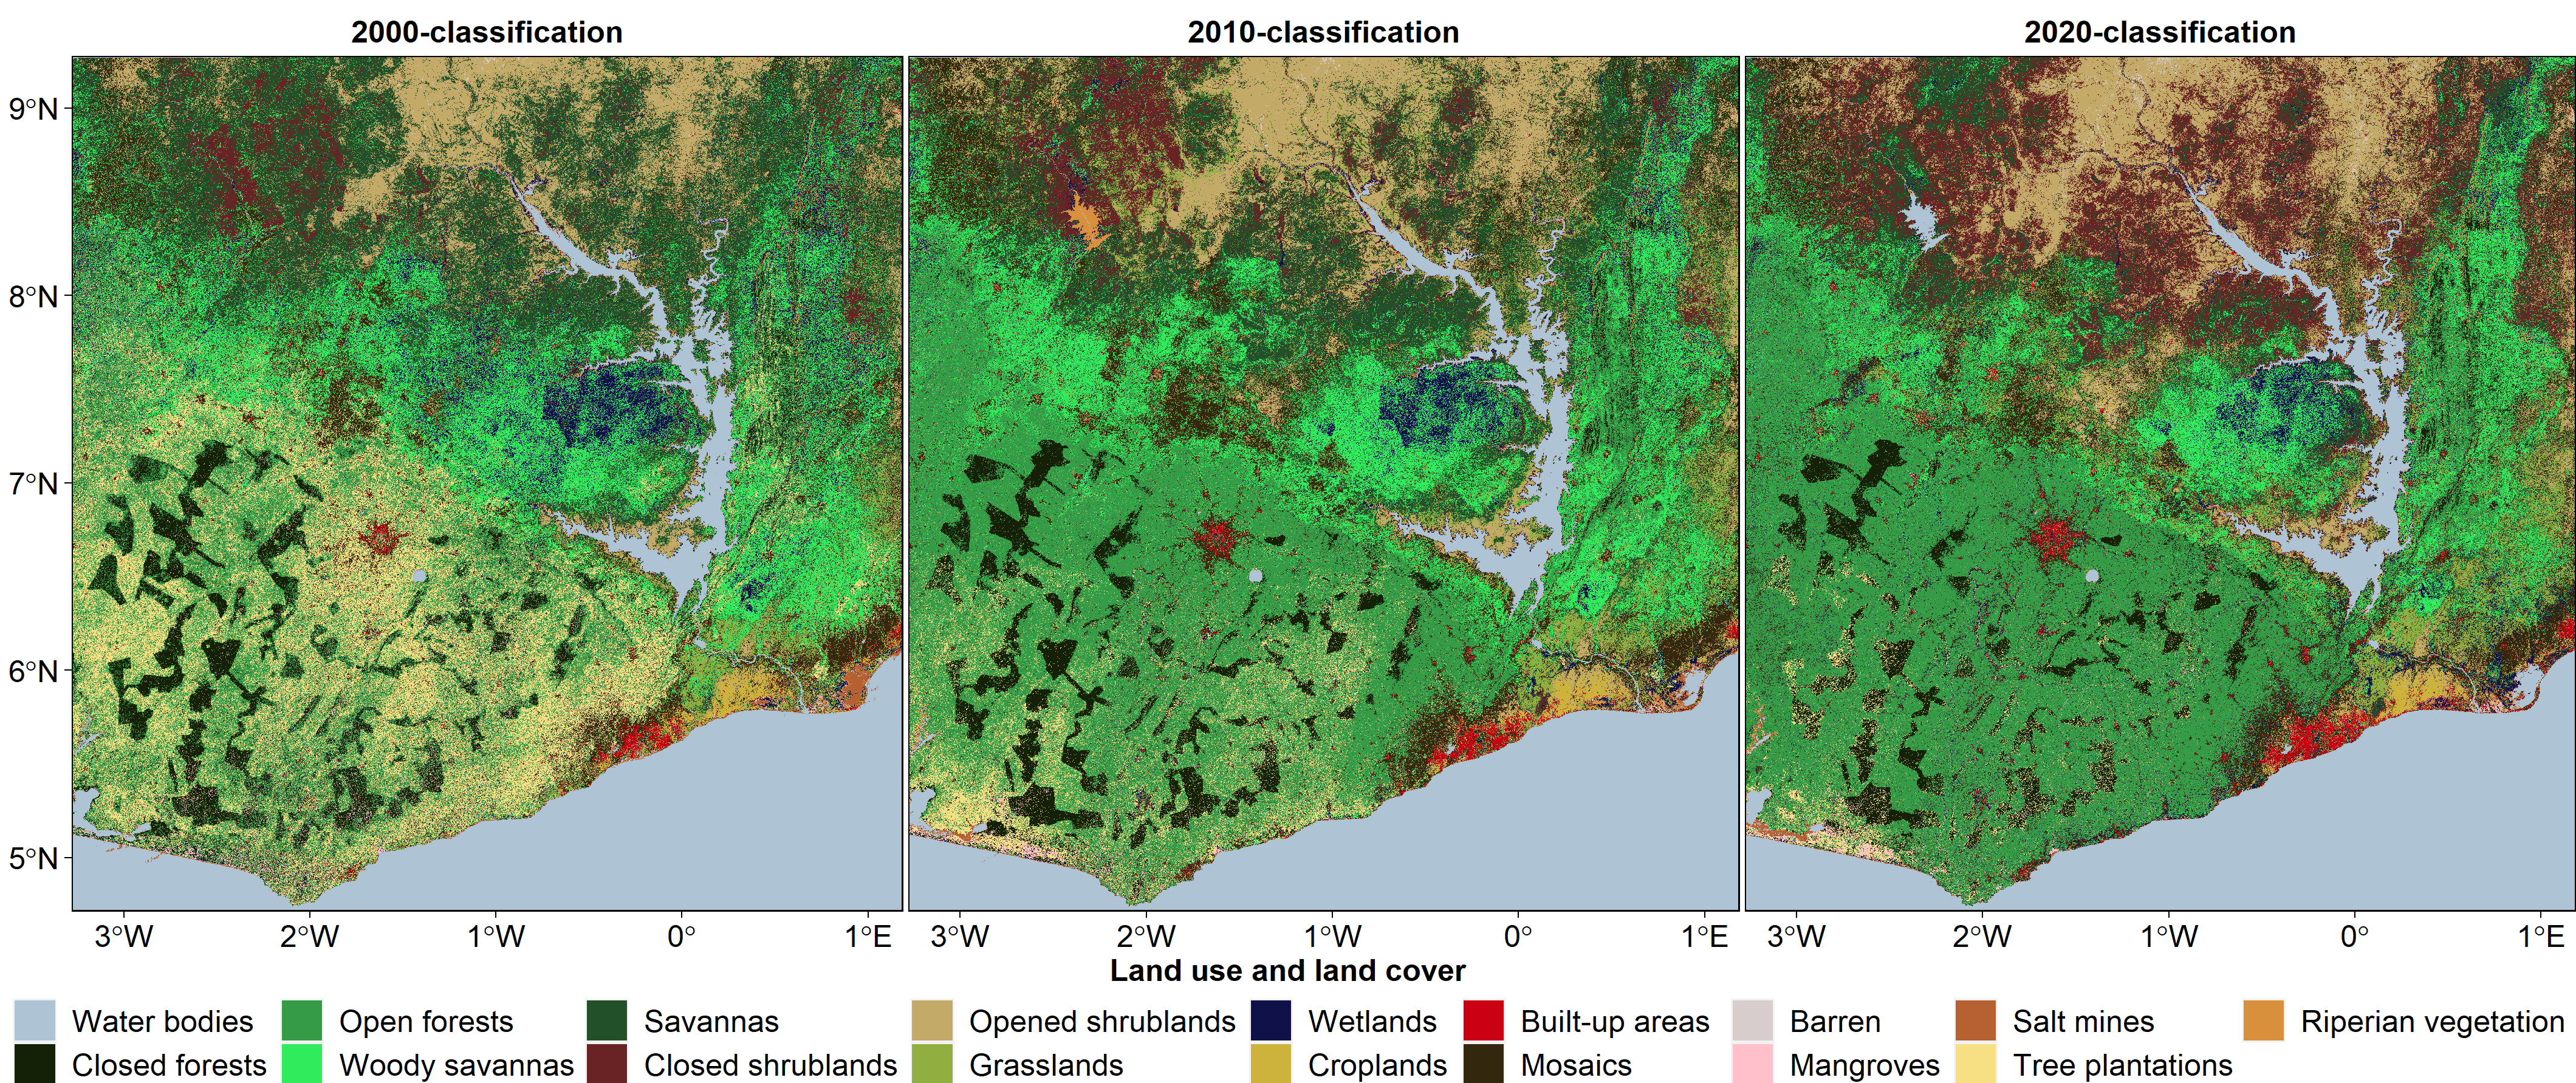
\includegraphics[width=1\linewidth,]{figures/pngs/Ghana_classifications} 

}

\caption{Multitemporal land use and land cover classifications of southern Ghana conducted for mangrove vegetation analysis. The input data were pre-processed using time series statistical models via harmonic modelling of all available Tiers 1 and Tiers 2 Landsat surface reflectance data acquired between 2000 and 2020. These classifications were based on random forest classifiers with a maximum number of 100 trees.}\label{fig:fig5}
\end{figure}

It appears from the LULC maps that closed forests have decreased over
time. This forest degradation, particularly noticeable over the portion
between 3\(^\circ\)W to 2\(^\circ\)W longitude and 5\(^\circ\)N to
6\(^\circ\)N latitude, appears to be higher upon the period 2010 to 2020
than during the previous decade. Water bodies appear to have remained
more or less stable, except for the appearance of some artificial
reservoirs such as the Bui dam on the course of Black Volta towards the
north. In the far most East towards the border with Togo, some salt
mines appear to have become water bodies suggesting a possible sea level
rise in this region. Built-up areas appear to have been increasing since
2000, suggesting an increased urbanization in the region. Mangroves
appear to be visible only in the West Coast around the border with Côte
d'Ivoire where they seem to have developed after the year 2000 since
they are less visible at glance in this region on the
2000-Classification. In Ghana, mangroves are generally of small size and
scattered along the coastline of the Atlantic Ocean.

\begin{table}

\caption{\label{tab:tab3}\label{tab3}Dynamics of major land use and land cover between 2000 and 2020 in Ghana. Data are reported in hectares of land. Change (2000 - 2020) is estimated by subtracting the 2020 estimates from the 2000 estimates. These changes are interpreted as slight (below 500,000 ha in absolute terms), moderate (between 500,000 and 1,000,000 ha in absolute terms), and high (above 1,000,000 ha in absolute terms).}
\centering
\resizebox{\linewidth}{!}{
\begin{tabular}[t]{>{\raggedright\arraybackslash}p{10em}>{\raggedleft\arraybackslash}p{12em}>{\raggedleft\arraybackslash}p{12em}>{\raggedleft\arraybackslash}p{12em}>{\raggedleft\arraybackslash}p{12em}}
\toprule
Land use and land cover class & 2020 & 2010 & 2000 & Change (2000-2020)\\
\midrule
Water bodies & 634,865.30 & 593,369.60 & 593,782.60 & 41,082.70\\
\addlinespace
Closed forests & 993,152.80 & 1,085,267.90 & 1,148,749.00 & -155,596.20\\
\addlinespace
Open forests & 4,940,904.00 & 4,440,366.00 & 2,854,193.00 & 2,086,711.00\\
\addlinespace
Woody savannas & 1,460,843.00 & 2,112,157.00 & 2,188,337.00 & -727,494.00\\
\addlinespace
Savannas & 1,439,506.00 & 2,386,865.00 & 2,997,046.00 & -1,557,540.00\\
\addlinespace
Closed shrublands & 2,124,826.10 & 866,632.00 & 529,264.90 & 1,595,561.20\\
\addlinespace
Opened shrublands & 1,986,620.00 & 1,722,579.00 & 1,516,987.00 & 469,633.00\\
\addlinespace
Grasslands & 769,840.20 & 861,989.00 & 360,629.30 & 409,210.90\\
\addlinespace
Wetlands & 797,702.80 & 536,080.60 & 836,869.00 & -39,166.20\\
\addlinespace
Croplands & 97,584.86 & 85,591.05 & 101,394.68 & -3,809.82\\
\addlinespace
Built-up areas & 171,858.60 & 112,050.20 & 117,516.60 & 54,342.00\\
\addlinespace
Mosaics & 1,475,992.00 & 1,612,346.00 & 1,172,785.00 & 303,207.00\\
\addlinespace
Barren & 74,014.78 & 20,345.02 & 20,845.76 & 53,169.02\\
\addlinespace
Mangroves & 52,691.18 & 46,587.36 & 121,475.94 & -68,784.76\\
\addlinespace
Salt mines & 28,082.26 & 31,541.75 & 50,014.97 & -21,932.71\\
\addlinespace
Tree plantations & 278,965.10 & 780,588.20 & 2,720,081.50 & -2,441,116.40\\
\addlinespace
Riperian vegetation & 93,552.30 & 126,645.15 & 91,028.86 & 2,523.44\\
\midrule
\addlinespace
Total & 17,421,001.28 & 17,421,000.83 & 17,421,001.11 & \\
\bottomrule
\end{tabular}}
\end{table}

Insights from image statistics revealed greater information than those
visible at glance (Table \ref{tab3}). There is a slight increase in
areas covered by water over the study period (2000 - 2020) which seems
to have mostly occurred upon the period 2010 to 2020. Closed forest area
has also slightly decreased even though this forest degradation appears
to progressively hold upon the study period. The area covered by the
open type of forests, in turn, has increased at a high rate over the
study period. This increase appears to have occurred at the expense of
closed forests with a similar rate over both study periods. Savanna
lands have experienced a high decrease with woody savannas being less
affected than savannas. While the decrease in woody savannas area
appears to have essentially occurred upon the period 2010 to 2020, the
decrease in savannas area appears to have been happening upon the entire
study period at an increasing rate. Shrubs, in contrast to savannas,
have been gaining land areas since the year 2000. Closed shrublands,
which show a higher increase rate than open ones, have experienced a
high increase while the increase in open shrublands has been moderate.
Cropland area appears to be stable, meaning that changes in agricultural
lands are fundamentally attributed to cropland and natural vegetation
mosaics which have seen a slight increase upon the period 2000 to 2010.
The area covered by tree plantations appears to have highly decreased,
particularly

\begin{table}

\caption{\label{tab:tab4}\label{tab4}Mangrove vegetation dynamics in relation to other land use and land cover between 2000 and 2020 in Ghana. Data are reported in hectares of land for both gains and losses. These gains and losses are interpreted as slight (below 5,000 ha), moderate (5,000 - 10,000 ha), and high (above 10,000 ha).}
\centering
\resizebox{\linewidth}{!}{
\begin{tabular}[t]{>{\raggedright\arraybackslash}p{9em}>{\raggedleft\arraybackslash}p{5em}>{\raggedright\arraybackslash}p{5em}>{\raggedleft\arraybackslash}p{5em}>{\raggedleft\arraybackslash}p{5em}>{\raggedright\arraybackslash}p{5em}>{\raggedleft\arraybackslash}p{5em}>{\raggedleft\arraybackslash}p{5em}>{\raggedright\arraybackslash}p{5em}>{\raggedleft\arraybackslash}p{5em}}
\toprule
\multicolumn{1}{c}{ } & \multicolumn{3}{c}{2000 - 2010} & \multicolumn{3}{c}{2010 - 2020} & \multicolumn{3}{c}{2000 - 2020} \\
\cmidrule(l{3pt}r{3pt}){2-4} \cmidrule(l{3pt}r{3pt}){5-7} \cmidrule(l{3pt}r{3pt}){8-10}
\textbf{Land use and land cover class} & \textbf{Gain} & \textbf{} & \textbf{Loss} & \textbf{Gain} & \textbf{} & \textbf{Loss} & \textbf{Gain} & \textbf{} & \textbf{Loss}\\
\midrule
Water bodies & 1,970.69 &  & 665.27 & 230.68 &  & 498.24 & 1,123.99 &  & 1,941.08\\
\addlinespace
Closed forests & 10,405.53 &  & 42,027.66 & 9,959.94 &  & 7,970.94 & 12,541.06 &  & 31,145.81\\
\addlinespace
Open forests & 4,245.51 &  & 24,445.83 & 2,070.32 &  & 3,556.10 & 7,395.80 &  & 37,435.64\\
\addlinespace
Woody savannas & 9.79 &  & 738.95 & 38.22 &  & 87.54 & 234.43 &  & 1,472.81\\
\addlinespace
Savannas & 11.74 &  & 257.18 & 43.20 &  & 19.75 & 147.05 &  & 546.29\\
\addlinespace
Closed shrublands & 23.96 &  & 182.41 & 5.69 &  & 8.98 & 42.81 &  & 416.11\\
\addlinespace
Opened shrublands & 7.90 &  & 255.83 & 34.96 &  & 41.17 & 95.57 &  & 1,127.07\\
\addlinespace
Grasslands & 11.42 &  & 361.62 & 32.55 &  & 7.47 & 302.02 &  & 506.06\\
\addlinespace
Wetlands & 1,448.30 &  & 4,211.22 & 2,613.68 &  & 922.08 & 2,563.10 &  & 5,602.48\\
\addlinespace
Croplands & 0.71 &  & 4.36 & 18.51 &  & 3.65 & 45.63 &  & 92.20\\
\addlinespace
Built-up areas & 29.53 &  & 346.73 & 50.15 &  & 98.79 & 340.14 &  & 1,274.09\\
\addlinespace
Mosaics & 46.19 &  & 1,780.36 & 267.37 &  & 336.17 & 1,002.19 &  & 7,111.21\\
\addlinespace
Barren & 5.60 &  & 82.22 & 23.04 &  & 92.88 & 55.66 &  & 1,656.30\\
\addlinespace
Salt mines & 1,521.19 &  & 1,711.93 & 357.76 &  & 642.00 & 438.68 &  & 2,104.20\\
\addlinespace
Tree plantations & 722.18 &  & 15,141.73 & 7,991.87 &  & 6,617.72 & 6,235.15 &  & 9,291.56\\
\addlinespace
Riperian vegetation & 2,383.93 &  & 5,519.47 & 4,139.16 &  & 869.84 & 3,979.60 &  & 3,604.72\\
\midrule
\addlinespace
Total & 22,844.19 &  & 97,732.77 & 27,877.13 &  & 21,773.31 & 36,542.88 &  & 105,327.64\\
\bottomrule
\end{tabular}}
\end{table}

\noindent between the years 2000 and 2010. Overall, mangrove vegetation
area has experienced a slight decrease upon the overall study period.
This mangrove degradation appears to have essentially occurred upon the
period 2000 to 2010. However, mangrove coverage seems to have increased
over the period 2010 to 2020, even though at a lower rate compared to
the previous decade.

\hypertarget{mangrove-vegetation-dynamics}{%
\subsection{Mangrove vegetation
dynamics}\label{mangrove-vegetation-dynamics}}

The overall assessment of mangrove areas dynamics shows that mangrove
vegetation experienced different trends in Ghana, with areas of
improvements and declines (Table \ref{tab4}). Examining the source of
mangrove areas dynamics, our results show that forests, wetlands,
cropland and natural vegetation mosaics, and tree plantations are the
top most important causes of mangrove losses. Mangroves have experienced
high gains at the expense of closed forests and moderate gains at the
expense of open forests, but neither the gain at the expense of closed
forests nor the gain at the expense of open forests has compensated for
the equivalent losses over the study period. Mangroves experienced high
losses in favour of closed forests and open forests. We observed
moderate losses in favour of cropland and natural vegetation mosaics and
tree plantations. While mangrove gains at the expense of tree
plantations compensated for the corresponding losses, mangrove gains in
relation to cropland and natural vegetation mosaics are much lower than
the corresponding losses. Even though in the range of minor loss,
substantial acreage of mangrove became barren, of which only less than a
tenth was recovered over the study period.

\hypertarget{site-specific-analysis-and-mangrove-change-direction}{%
\subsection{Site-specific analysis and mangrove change
direction}\label{site-specific-analysis-and-mangrove-change-direction}}

The findings of the LULC analysis provide useful insights into the
overall dynamics of LULC in the coastal regions of Ghana. In this
section, we attempt to provide further information for operational
application in mangrove conservation by identifying areas of mangrove
increase and decline in a spatially explicit manner. Herein, we present
the major mangrove areas of Ghana in some sort-of case studies for
conciseness and better visualisation. For a complete picture of mangrove
dynamic in Ghana, we refer the reader to the technical materials (see
Software and data availability). We presented 10 different cases
covering most of the major mangrove areas of Ghana. These include urban
mangrove vegetation, those found around rivers, and those found around
lagoons. Despite the declining trend observed over the past decade, many
of these areas appear to generally exhibit a stable trend during the
last decade.

Mangrove coverage in the West Coast of Ghana appear to have remained
dominantly stable over the study period, particularly during the period
2010 to 2020 (Figure \ref{fig:fig6}). Major spots of this stability are
found around the trench between Tikobo 1 and Aiyinase through Amansuri
Lake. This area has seen important mangrove expansion before 2010,
period after which the area seems to have dominantly stabilised. While
most of the area exhibits a stable trend, several spots show a declining
trend in mangrove vegetation cover suggesting that the area tends
towards a decline. Beyond Tikobo 2 to the north, however, only small
patches of mangroves remain before 2000, period after which these
mangroves were converted into other LULCs. Other spots of mangrove
degradation are found around Half Assini where most mangroves seem to
have disappeared over the last decade. Slightly to the south of Half
Assini, mangrove coverage appears to have substantially increased over
the study period.

In the vicinity of Kpani river, mangrove coverage essentially remained
stable over the study period, with localised spots of decrease and
increase (Figure \ref{fig:fig6}). In the Kpani River basin, localised
spots of mangrove area expansion are encountered in southeast of Miemia
along the left branch of Kpani River as well as in the north of Lake
Ehunli Lagoon along

\begin{figure}[!htbp]

{\centering \includegraphics[width=1\linewidth,]{figures/pngs/Ghana_mangrove_change_direction} 

}

\caption{Dynamics of mangrove vegetation in selected mangrove areas of Ghana.}\label{fig:fig6}
\end{figure}

\noindent the right branch of the Kpani River. The regeneration near
Miemia seems to have essentially taken place during the period 2010 to
2020. Minor mangrove coverage expansion is observed in the southern
shore of Ehunli Lagoon, but the mangrove area around the lagoon seems to
be in decline over the study period. Beyond the proximity of Kpani River
and Lake Ehunli Lagoon, the mangrove area appears to have been
substantially declining long before 2000, leaving only a few patches
scattered all over the region. These mangrove remains seem to have
mostly been converted into other LULCs after 2010. Kpani River presents
a similar trend of stability compared to Ezile River near Akwidaa (not
presented here). However, in Ezile River, the regeneration appears to be
negligible compared to the degradation affecting most of the landmass
between Akwidaa and Dixcove. In this area where little has been gained,
the stability of the mangrove area is limited to the riverbank, beyond
which mangroves are essentially in decline over the study period.

Along Butre River and its upper tributaries on either side of the river,
mangroves appear to have regenerated between 2000 and 2010. In the lower
tributary giving rise to the eastern floodplain, mangroves appear to
have predominantly decreased at the periphery of the floodplain which
represent the hotspot of Butre River mangroves. Both areas of gain and
loss appear to have kept the same trend between 2010 and 2020, even
though at a lower rate compared to previous decade. Further to the East
of Butre River in Takoradi town, mangroves appear to have substantially
declined over the study period (Figure \ref{fig:fig6}), despite the few
stable mangrove spots around water bodies. Except for the few spots of
stability around water bodies, mangroves in Takoradi town of Ghana
appear to have substantially declined over the study period (Figure
\ref{fig:fig6}). Mangrove area in this region seems to have declined
even before 2000. Close to the water bodies, we noticed both areas of
stability, decline and increase, but mangrove area increase and decline
appears to be only limited to the immediate proximity of these urban
water ways. These remaining mangrove areas, however, seem to remain
stable with a few regeneration patches over the period 2010 and 2020.

For the most, mangrove area around Pra River kept a stable trend over
the study period (Figure \ref{fig:fig6}). Mangrove area has remained
dominantly stable on either side of Pra river, particularly in the
immediate proximity of the Atlantic Ocean. Mangrove area seems to have
increased in some areas close to the Atlantic Ocean directly below
Fawumaye. This regeneration gradient appears to circumvent Fawumaye
following an arc reaching up to the northern part of the town. Beyond
this point, only few patches of mangroves remain before 2000, period
after which they have mostly disappeared. The same situation is observed
around Assako Essaman. Another spot of regeneration is observed directly
below Assako Essaman on the shore of Atlantic Ocean. In this relatively
small area, mangrove area appears to have increased during the last
decade, essentially compensating for the lost they have seen over the
period 2000 to 2010.

In Cape Coast town of Ghana, mangrove area shows a stable trend with
many spots of increase, suggesting that mangrove vegetation have seen an
interesting regeneration over the study period (Figure \ref{fig:fig6}).
While our results are not conclusive regarding the situation of mangrove
vegetation in the town before 2000, the consistent declining trend
observed over all mangrove areas along with the few spots of decline
across the town during the last decade suggest that some mangrove areas
were converted into settlement long before 2000. This is supported by
the declining trend near Amamoma where mangroves appear to have
undergone important degradation following the ongoing urban expansion in
Amamoma belt of Cape Coast.

This settlement encroachment appears to have started long before 2010.
The mangrove area appears to have considerably shrunk over the last
decade, suggesting that these mangroves are likely to disappear in the
near future. Other spots of mangrove decline in Cape Coast town of Ghana
are found around Fosu Lagoon where most of the surrounding mangroves
have been converted over the study period. However, the overall mangrove
area appears to have increased over the last decade in Cape Coast.
Except for Fosu Lagoon, stable to increasing trend appears to prevail in
most mangrove sites over the period 2010 to 2020. Upon this period, the
remaining mangroves near Amamoma remained dominantly stable while those
in Benya Lagoon were inclined towards an increasing trend.

Mangroves in Narkwa region have experienced important decline during the
period 2000 to 2010 (Figure \ref{fig:fig6}). Except for a few spots
showing stable to increasing trend in Amisa Lagoon, almost all mangrove
in the region were depleted during this period, particularly in Narkwa
Lagoon. However, substantial mangrove areas have recovered over the last
decade. Along the land mass spanning from Anboko to the eastern parts of
the twin Ekumfi through Ankaful, only a few spots of decline are
observed in 2020. This mean that mangroves in the region have
essentially recovered from the important degradation that took place
during the previous decade. Overall, the region appears to have gained
appreciable mangrove coverage in Amisa Lagoon near Ankaful as opposed to
Narkwa Lagoon showing a leading trend of mangrove degradation.

The dynamics of mangrove area in Muni Lagoon is dominated by an
increasing trend over the study period (Figure \ref{fig:fig6}). This
area appears to be deprived of mangroves vegetation before 2010. The few
spots of mangrove degradation around the lagoon and along the coastline
in the East of the lagoon during the period 2000 to 2010 suggest that
mangroves have experienced an unprecedent decline before 2000. The
current mangrove vegetation in the lagoon dates back to no more than
2010 since no mangroves were observed before 2010 in the lagoon.

Like in Muni Lagoon, an increasing trend dominated the neighbouring
Ayensu River. In this area, however, mangroves vegetation dates back to
2000, meaning that some mangrove areas remained stable over the study
period. Beyond the lower tributary of Ayensu River to the East, however,
substantial mangrove areas appear to have emerged at the expanse of salt
mines. This area has seen important mangrove regeneration over the last
decade.

In Accra town of Ghana, mangrove area appears to have increased over the
study period (Figure \ref{fig:fig6}). Most mangrove areas between Densu
and Kepsi Lagoon appear to exhibit stable trends, with the majority of
them inclined towards an increase. Mangrove area gains are observed all
over Densu region (Densu River and Densu Estuary including Densu Salt
Mines). These mangrove area gains appear to have taken place in the
western part to consistently progress northwards. In this area where we
observe important mangrove regeneration, mangroves appear to have gained
substantial land areas at the expanse of salt mines. Except for a few
spots of declines, mangrove area appears to have increased over the
banks of Densu River.

In Densu region, area of mangrove loss appears to be limited to Densu
Estuary, particularly at the periphery of Densu Salt Mines where
substantial losses in favour of settlements are observed from nearly
Mallam Mosque up to the upper border of Densu Salt Mines. The lower part
of the estuary (between the lower border of Densu Salt Mines and the
shore of Atlantic Ocean) shows a mixture of stable, increasing and
declining mangrove areas over the study period. Despite a few spots of
decline, mangrove area appears to have increased over the study period
in Korle Lagoon. Mangrove area has shrunk in favour of settlements in
the left branch of Kpeshi Lagoon whereas this area has essentially
expanded over the right branch and the lower part of the lagoon.

In Accra, mangrove area appears to have seen important decrease over the
decade 2000 to 2010 with major mangrove areas, including Densu estuary,
Korle Lagoon and Kpeshi Lagoon, exhibiting a stable to declining trend
of mangrove vegetation. Only a few spots of mangrove area increase,
essentially in Densu Estuary and Kpeshi Lagoon are observed between 2000
and 2010. It appears that most of the mangrove vegetation in Densu River
has emerged after this period. Except for relatively minor loss due to
urbanisation that appears to continuously encroach on mangrove area,
mangrove vegetation has widely spread over the last decade, resulting in
Densu region and Korle Lagoon exhibiting increasing trends, and Kpeshi
Lagoon showing stable to increasing trend in mangrove area.

The land portion between Laiwi and Moyio lagoons of Ghana is a
dominantly an agriculture region where croplands extend to the coastline
of Atlantic Ocean. In this region, mangrove vegetation appears to be
tightly limited to the immediate proximity of lagoons and coastline
(Figure \ref{fig:fig6}). Mangrove vegetation appears to have increased
everywhere around lagoons and along the coastline between Laiwi and Moyo
lagoons over the study period. Except for relatively minor losses
scattered over the region, we only noted a few spots of stable mangrove
vegetation mostly over abandoned salt mining areas.

Given the presence of a few scattered tickets of mangrove vegetation
before 2000 and the absence of these in 2010, we presume that mangrove
vegetation in the region was depleted before 2010. Essentially, these
mangroves appear to have regenerated during the last decade.

The Eastern Coasts of Ghana show both increasing and stable trends in
mangrove area, along with areas of stable mangrove vegetation over the
study period. In general, however, mangrove area appears to have
increased in the western part of the region. Spots of decreasing
mangrove areas, which appear to augment northwards, are mostly
encountered in the central part of the region. In the western part,
mangrove area appears to have increase around Lake Songaw Lagoon where
we only observe a few declining spots at the periphery of the lagoon. In
the central part, mangrove area appears to have decreased in volta River
and the western part of Volta Estuary. In this part, we only observe a
few stable to increasing trend of mangrove vegetation towards the shore
of Atlantic Ocean. Mangrove vegetation in the eastern part of Volta
Estuary, where we observe consistent mangrove stability over a large
area between the estuary and Keta Lagoon, appears to have remained
stable or increased over the study period. Relatively fewer mangroves
are observed towards the Togolese border around Keta Lagoon where most
of these appear to show an increasing trend with a few spots of decline.

Mangrove regeneration in the Eastern Coasts of Ghana appears to have
fundamentally taken place during the previous decade. Essentially,
mangrove vegetation appears to be depleted before 2000 in Lake Songaw
Lagoon where we only observe a few spots of this vegetation by 2000.
Most of this vegetation appears to have regenerated during the previous
decade. Mangrove area, which appears to have shrunk between the eastern
part of Volta Estuary and Keta Lagoon during the previous decade,
appears to have increased over the last decade. In contrast, mangrove
vegetation appears to be in progressive decline over the study period in
Volta River and the western part of Volta Estuary where some areas
remained stable since 2000.

\hypertarget{discussion}{%
\section{Discussion}\label{discussion}}

The approach we presented addresses key issue related to optical remote
sensing, LUCC classification, and post-classification change detection.
By reconstructing gap free times series at the nominal spatial
resolution in a context of persistent cloud cover, the approach presents
clear advantage for a wide range of remote sensing applications. On the
one hand, the high classification accuracy we have achieved, despite a
high number of LULC classes and validation samples, results from the
ability of the approach to account for the history of pixels without
accounting for random noise. On the other hand, the use of unsupervised
classification to constrain the reference data over pixels of persistent
LULC have contributed to this high accuracy. This approach can be almost
always useful for remote sensing-based analysis, particularly in
situations of limited resources and limited access to study sites. One
limitation can be expected for pixels that undergone LULC change over a
reference period for it can be confusing to which LULC it would be
classified \citep{Zhu-and-Woodcock-2014}. Obviously, this has not been
of major concern in this study and is unlikely to constitute a problem
as long as the reference period is wisely chosen. With a short and odd
number of years as reference periods (i.e., 3 successive years) in our
case, the distribution of any changed pixel would be skewed towards of
the most likely characteristic LULC class. The random forest algorithm
can then handle such situation without any ambiguity, particularly when
the images in the time series are spread across multiple bands. In any
case, the reference period should be chosen in a way to avoid capturing
multiple changes while allowing the time series to capture enough data
for the classification algorithm to find windows for discriminating
pixels of different classes.

In the coastal regions of Ghana, the chance of getting clear Landsat
observation appears to increase eastwards (Figure \ref{fig:fig1}). From
the result of mangrove dynamics, it becomes clear that the ability of
the model to remove random noise depend on the amount of available clear
observations. This is reflected by the presence of potentially noisy
pixels in some of the change maps (i.e., Amansuri Lake, Kpani River,
Butre Estuary) presented in Figure \ref{fig:fig6}. This noise decreases
in space form West to East as more clear observations become available.
It also decreases in time from the earliest to the most recent change
map as more data become available with the availability of different
Landsat sensors. One way to reduce this noise is to use the model
by-products (e.g., phase and amplitude, harmonic coefficients) described
in equation \eqref{eq:1} as part of the classification inputs. Future
works may also consider the use of normalized difference spectral
indices (e.g., NDVI, NDWI) along with these model by-products to improve
the estimates. With a few caveats, the increasing availability of
synthetic aperture radar data presents another opportunity to improve
these estimates. PALSAR-2/PALSAR (as yearly mosaic since 2007) and
Sentinel-1 (as 12 days temporal resolution since 2015) data are
currently freely available for Ghana from Google Earth Engine.

The results of mangrove dynamics expose the major mangrove areas of
Ghana, each of which having its own peculiarity. In Ghana, it seems that
mangrove degradation was perceptible long before 2000 and has triggered
a massive replating campaign along the coast. This led to the formation
of organized groups engaged in systematic planting and harvesting of
mangrove trees. While regeneration of mangroves in most areas is due to
replanting, the causes of their degradation is more context specific
even though they mostly relate to overexploitation. Despite the
noticeable impacts of the replanting projects in many areas along the
coast of Ghana, genuine support from local community towards these
projects has remained largely unclear
\citep{Aheto-et-al-2016, Asante-et-al-2017}.

The spatial distribution of gain and loss in mangrove vegetation in
Butre River suggests a possible increase of salinity in the lower
tributary since mangroves regeneration appear to increase with lower
order tributaries. Regardless the cause, the pattern of loss and gain
paints some sort of mangrove migration from the lower part to the upper
part of the river. This is likely to result into an overall decrease of
mangrove vegetation in the area since the potential area for mangrove
development is higher in the lower basin. In urban areas (e.g.,
Takoradi, Accra), the main drivers of mangrove degradation are urban
encroachment and pollution. The general pattern of mangrove degradation
in these urban centres relates to population density in relation to the
carrying capacity of the mangrove area, as in the case of Takoradi and
Ayensu River. The closer the mangrove area to settlement, the more
likely the degradation, and the larger the agglomeration, the more
likely the degradation. The depletion of mangrove in Muni Lagoon, for
instance, can be mainly explained by the range of mangrove exploitation
in relation to the carrying capacity of the mangrove. In this area,
mangroves were intensively use as source of domestic and commercial
charcoal and firewood while being subjected to other practices (e.g.,
bush burning, agricultural encroachment, unsuitable fishing) that are
conducive to their degradation \citep{A-Rocha-Ghana-2016}. In Densu
River, mangrove degradation is mainly due to increase urbanisation which
resulted in the encroachment of mangrove areas, the dumping of waste
into the river along with excessive fishing and oysters harvesting. In
Volta Estuary, mangrove degradation stemmed from uncontrolled access to
mangrove resources but the failure of mangrove restoration programmes is
mainly due to issues related to governance and tenure along with the
local perception of mangroves as a mean for economic gain rather than a
mean for environmental conservation
\citep{Asante-et-al-2017, Ashiagbor-et-al-2021}.

In a nutshell, we identified 5 major groups of factors involved in
mangrove degradation in Ghana.

\begin{enumerate}
\def\labelenumi{\arabic{enumi}.}
\item
  Global changes including infrastructural development, urbanization and
  climate change. For example, the construction of the Akosombo dam of
  the Volta river negatively affected the agricultural and fishery
  sectors in the Volta estuary, resulting in increased cutting of
  mangroves by the local to make a living
  \citep{Aheto-et-al-2016, Feka-and-Ajonina-2011, Rubin-et-al-1999}.
  Increased level of industrial and domestic wastes due to urbanization
  generally results in the pollution of water sources near cities. This
  is the case of Korle Lagoon which drains most of the untreated waste
  of Accra into Atlantic Ocean. This pollution, causing the
  proliferation of invasive species, the reduction of oxygen level and
  increasing the level of salinity, is particularly a problem for
  mangrove trees in Korle Lagoon \citep{Boadi-and-Kuitunen-2002}.
\item
  Local awareness including local perceptions and the erosion of
  cultural and religious beliefs associated with coastal resources. Such
  examples are the cases of out-of-taboo fishing in Fosu, Muni and
  Songor lagoons \citep{Darkwa-and-Smardon-2010, Ntiamoa-Baidu-1991},
  the perception that the mangroves of Fosu Lagoon shelter dangerous
  species such as snakes \citep{Darkwa-and-Smardon-2010}, or the
  drainage of urban waste into mangroves swamps in Accra
  \citep{Essumang-et-al-2012}.
\item
  Land tenure regime including the sense of ownership. Mangroves lease
  often goes for a period of 10 years, resulting in increased tree
  cutting by the lessee \citep{Armah-et-al-2009}.
\item
  Legislation, governance and policy including the lack of enforcement
  for mangrove resource protection {[}\citet{Armah-et-al-2009};
  Feka-2015{]}. Despite the various conservation projects tailored to
  mangroves ecosystems in Ghana, these mangroves remain vulnerable to
  anthropogenic disturbance as they lack a clear legislation that could
  protect them from overexploitation \citep{Asante-et-al-2017}.
\item
  Lucrative including commercial wood cutting, agricultural expansion or
  salt mining. Examples of such are the conversion of mangroves into
  salt pans and urban encroachment in Keta Lagoon
  \citep{Asante-et-al-2017}, charcoal and firewood for fish smoking in
  Fosu Lagoon \citep{Darkwa-and-Smardon-2010}. \citet{Aheto-et-al-2016}
  estimated the annual net income per hectare of mangrove wood to
  approximate \$4824.88 for traders and \$383.12 for planters.
\end{enumerate}

Further study on the nexus between people and their mangrove across the
whole country would provide interesting insights for conservation
policies. Mangrove restoration can be expansive as it does not only
require the replanting of thousands of mangroves trees but more
importantly their maintenance and reaching thousands of people. The key
aspect to keep in mind is that mangroves degrade more as result as a
lack of environmental education (e.g., awareness of common resource and
conservation issue, and strong management skill at a general public
level) than they do due to natural factors. Mangrove restoration would
require, in the first place, a large-scale training of the locals on
sustainable use and management of the mangrove. Amongst other things,
mangrove restoration in Muni required the inclusion of all communities
(e.g., Mankoadze, Biwadze and Akosua Village) whose activities impact
the mangrove, a number of training sessions including, tree nursery as a
mean to avail mangrove seedlings, mangrove management and conservation
to strengthen the local skill in mangrove planting and maintenance, the
use and making of efficient fuel stoves to reduce deforestation due to
wood fuel.

Although the social dimension may be more crucial than the ecological
one for mangrove conservation, mangrove conservation policies should
also consider the biophysical settings in which mangroves evolve.
Lagoons rely on water supplies from both the ocean and some source of
fresh water (e.g., rivers) which must be at an adequate proportion to
allow the development of certain mangrove species. It is important to
keep the salinity at a relatively low level, particularly for white
mangrove such as Avicennia species. In this case, alternative management
model would consider a proper maintenance of fresh water sources as a
crucial aspect of management and conservation. An option of such
management would be river bank hedging. A hedgerow of tree along the
river would protect the river from erosion and sedimentation, and reduce
evaporation to insure better fresh water supply to the lagoon.

\hypertarget{conclusion-and-recommendations}{%
\section*{Conclusion and
recommendations}\label{conclusion-and-recommendations}}
\addcontentsline{toc}{section}{Conclusion and recommendations}

This study addresses several issues concerning LULC classification,
particularly when the classification outputs are intended for LULC
change detection. We discussed how cloud cover can have important
implications for LULC classification in the coastal regions of Ghana and
demonstrate how time series statistical models can be used to curate
this problem. Currently, Landsat mission is the best publicly available
source of data that provides sufficient records for studying decade-long
LULC pathways in a comprehensive manner. We argue that continuous time
series analysis is more likely to provide unbiased LULC classification
than single point image analysis. Due to various remote sensing
artifacts, however, the temporal resolution of usable Landsat data is
often insufficient for continuous time series analysis. To address this
challenge, our approach consisted in capturing the inherent landscape
phenology into time series statistical models that feed on the few
usable information to construct gap-free time series for image
classification. In regard to this issue, future research direction would
be the use of both spatial and temporal relationships between pixels to
infer missing data. Such analysis should consider harmonizing pixel
level data such that these are comparable across spatial and temporal
domains. In this study, we discussed the issue of training data and
classifiers, which need to be comparable across the temporal scale of
change detection analysis. While we have not conducted formal analysis
in regard to the effects of these aspects on our results, it appears
that they have substantially contributed to the high statistical
accuracy observed in our classifications. Although the traditional
confusion matrix provides formal estimate of map accuracy in a variety
of statistical metrics, studies dealing with LULC classification should
always cross-check the reliability of these metrics to ensure that maps
reflect the ground conditions. In this regards, future research
direction would be the use of probabilistic models to report class
detection probabilities. Such exhaustive accuracy measures would be more
convenient and realistic in the sense that they estimate pixel-level
accuracy, rather than class-level accuracy as does the traditional
confusion matrix. Ecological studies aiming at LULC classification and
change detection can greatly benefits from the use of continuous Landsat
records and the other important considerations addressed in this study.
This can be particularly important when the signature of the target LULC
classes are similar. While mangroves represent our class of interest in
this study, their spectral signature is often similar to that of many
forest LULC classes found in the study area. This means that they can be
easily mis-classified, in which case the classification error would
propagate into change detection. In such a case, the use of continuous
time series becomes a necessity rather than a luxury since it offers a
rich data record for distinguishing between similar LULC via their
phenological profiles. The analysis of LULC dynamics show that LULC are
subject of important conversion in the coastal regions of Ghana. Future
research directions would be to examine these LULC conversions. Such
studies may seek to understand which LULC are expanding, document which
LULC are shrinking as result of this expansion, estimate the rate at
which the expansion is taking place, and investigate the main drivers of
these LULC conversions. In this study, we attempted to provide such
information for mangrove vegetation and identify areas of mangrove
decrease and increase. Based on the results of our analysis, we
recommend large scale mangrove restauration in Ghana. Failure to do so
is likely to result in the loss of many mangrove areas, particularly
those in the vicinity of urban centres. The first step towards such a
restauration program should be the zoning of priority areas, the
quantification of the costs and benefits in forms of spatially explicit
ex-ante impact assessment, and the definition of near and far futures
milestones for mangrove development impacts. Future research for
mangrove changes analysis in the coastal regions of Ghana would be the
quantification of the change magnitude and the development of remote
sensing-based indicators of mangrove vegetation change and mangrove
vegetation quality. In all these cases, the use of spatially explicit
statistical model capable of reconstruction high temporal frequency of
comparable pixel data that accurately describe landscape-level phenology
of LULC provides a powerful tool for analysing changes in LULC.

\hypertarget{acknowledgements}{%
\section*{Acknowledgements}\label{acknowledgements}}
\addcontentsline{toc}{section}{Acknowledgements}

This research was supported by the American People through the United
States Agency for International Development (USAID) under the
BAA-AFR-SD-2020 Addendum 01, (FAA No.~7200AA20FA00031). The contents of
this manuscript are the sole responsibility of the authors and do not
necessarily reflect the views of USAID or the United States Government.

\renewcommand\refname{References}
\bibliography{bibliography.bib}


\end{document}
